\section{Results}

\subsection{Cloud-proximity phenomenology}
\label{sec:result-cld_dist}

% Lead with the observation:

% - XCO2 anomaly versus cloud distance;
% - positive near-cloud response over land and negative response over ocean;
% - characteristic land-r15 and ocean-r05 distance scales;
% - quality-flag composition and observation loss with cloud distance.

% This result establishes the problem before introducing correction skill.

We analyze the $17.75$M footprints from the 2016-2020 analysis set (Sect.~\ref{sec:method-daataset-split}) with a valid nearest cloud distance. $41.7\%$ of all footprints lie within 4 km of the nearest detected cloud ($60.7\%$ within 10 km). We use $d_0 = 10$~km as the reference to calculate the \xcobc anomaly ($\Delta \mathrm{X_{CO2}^{B11}}$), as shown in Fig.~\ref{fig:OCO-ocean-land-cld_dist}a. The results demonstrate that $\Delta \mathrm{X_{CO2}^{B11}}$ is opposite in sign, with negative over ocean and positive over land before any correction is applied. Furthermore, the ocean response has decayed by $\thicksim5$ km, well inside the threshold, whereas the land response is still $\thicksim0.5$ ppm when the 10-km reference cut truncates it by construction. In other words, the cloud-influence distance could be different over ocean and land. As a result, we set the new reference distances separately with $d_0 = 5$~km for ocean and $d_0 = 15$~km for land.



\begin{figure}[t]
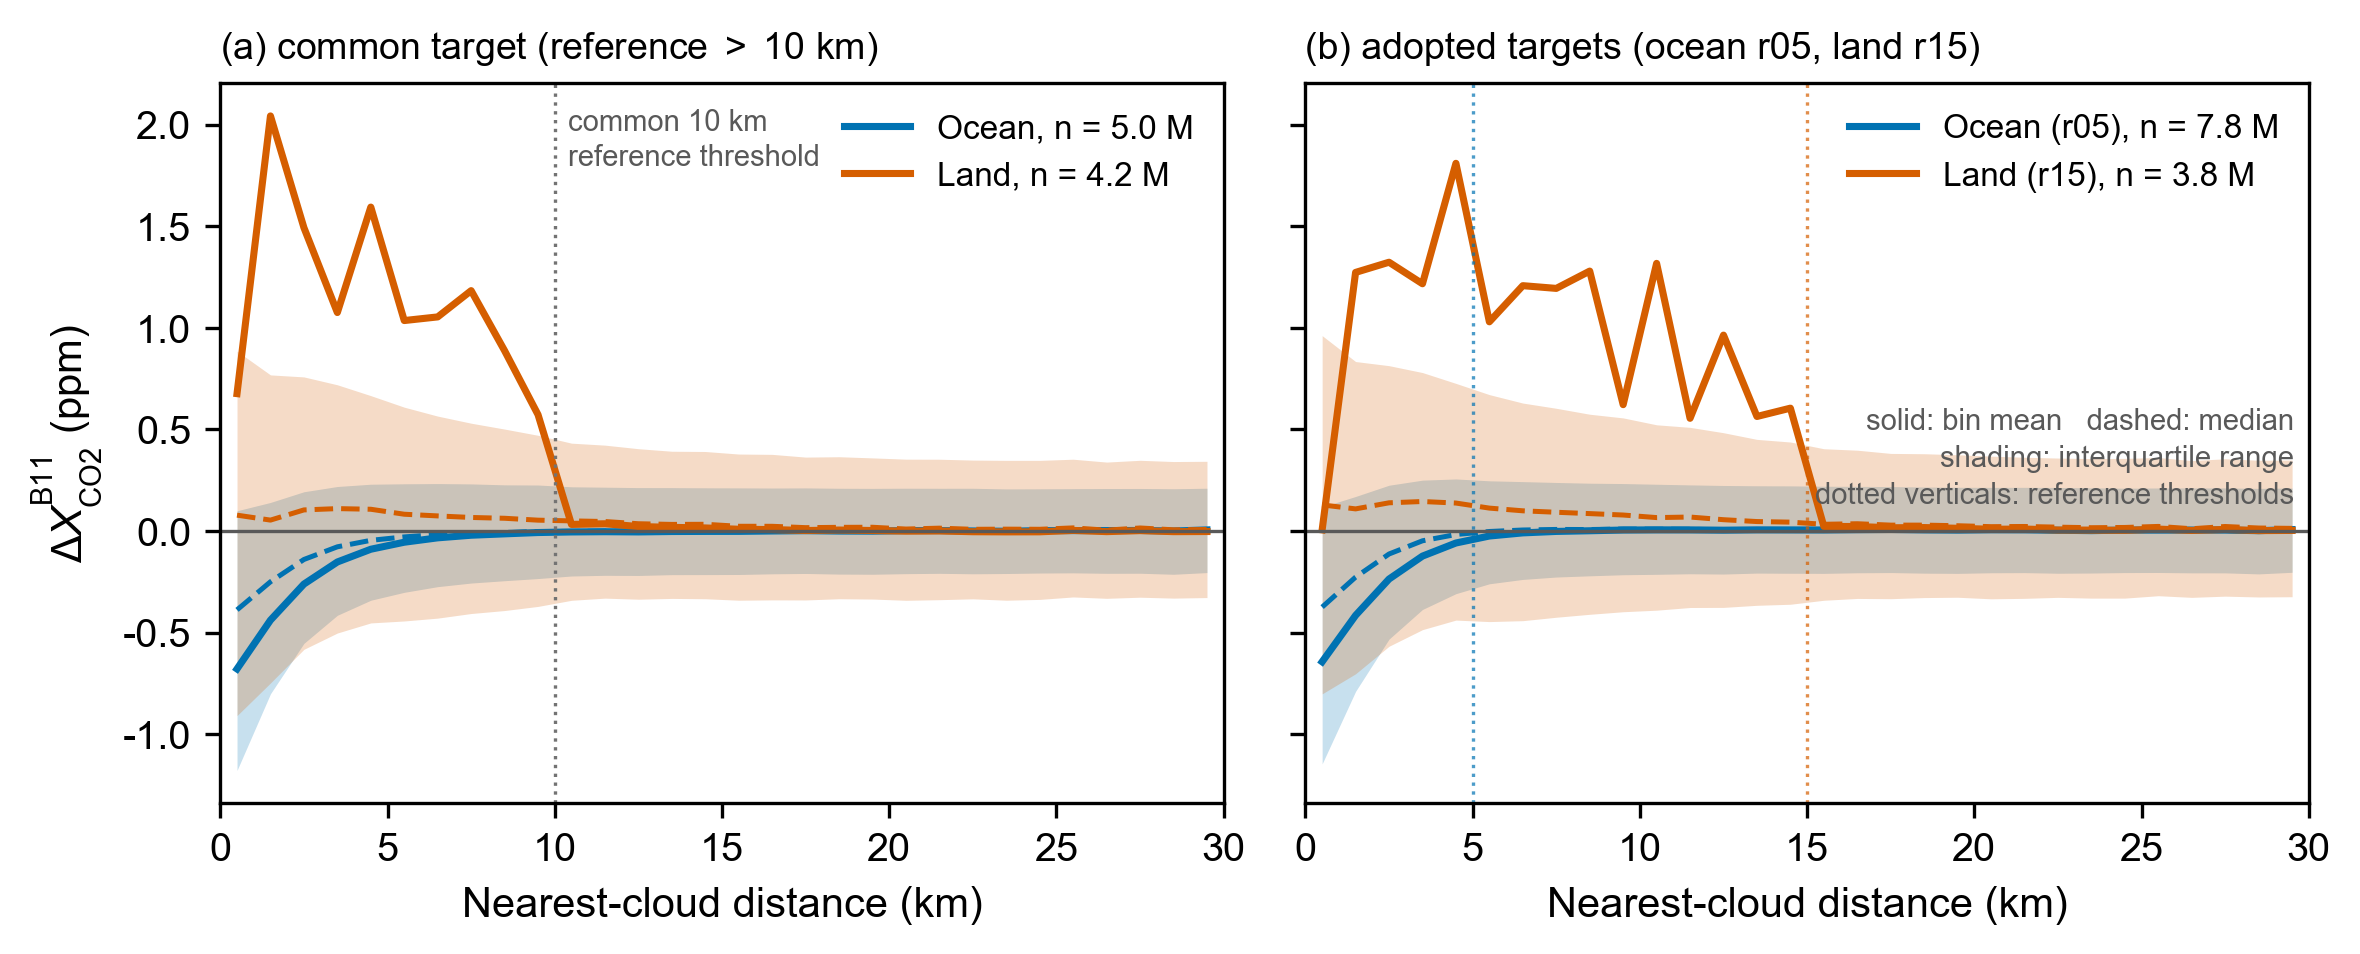
\includegraphics[width=\textwidth]{figures/fig03_anomaly_decay.png}
\caption{Within-orbit clear-sky \xco anomaly versus nearest-cloud distance for the 2016–2020 analysis set (116 dates; 1-km bins). (a) Both surfaces under a common anomaly target whose clear-sky reference lies beyond 10 km. The common threshold is too tight for land and unnecessarily wide for ocean, motivating the surface-specific radii. (b) The adopted production targets with ocean referenced beyond 5 km (r05, n = 7.8 M) and land beyond 15 km (r15, n = 3.8 M). Solid lines show the bin mean, dashed lines the median, and shading the interquartile range: over ocean the whole distribution shifts negative near cloud, whereas over land the mean far exceeds the nearly unmoved median. The land bias is carried by a skewed tail of strongly affected soundings rather than a shift of the full population.}
\label{fig:OCO-ocean-land-cld_dist}
\end{figure}


After recalculating $\Delta \mathrm{X_{CO2}^{B11}}$, the land response indeed persists to $\thicksim15$ km, and the ocean curve is unchanged (Fig.~\ref{fig:OCO-ocean-land-cld_dist}b). The dotted lines mark each reference threshold, beyond which the anomaly returns to zero by construction. The signature of opposite sign of ocean and land $\Delta \mathrm{X_{CO2}^{B11}}$ also remains the same. 59.1\% of ocean footprints are within the 5 km ocean target radius, and 46.8\% of land footprints are within the 15 km land target radius. We use the newly calculated $\Delta \mathrm{X_{CO2}^{B11}}$ with $r05$ for ocean and $r15$ for land in later analysis and training.

\subsection{Spectral features and cloud distance}
\label{sec:result-spec_anal}


We derive the spectral features by fitting from three OCO-2 bands, as described in Sect.~\ref{sec:methods_photon_path}. The land footprints are categorized as various surface types based on the MODIS yearly land cover type product (MCD12C1). We compare the average difference of each variable from near-cloud and far-cloud footprints (nearest cloud distance < $5$~km for ocean and <$15$~km for land). For each surface class $g$ and reference-corrected spectral variable
$\Delta v$, the near-cloud effect size shown in Fig.~\ref{fig:land_type_features} is the
far-field-normalized difference
%
\begin{equation}
  E_z(\Delta v, g) \;=\;
  \frac{\overline{\Delta v}_{g}^{\,\mathrm{near}}
       - \overline{\Delta v}_{g}^{\,\mathrm{far}}}
       {\sigma_{g}^{\mathrm{far}}(\Delta v)} ,
  \label{eq:effect-size}
\end{equation}
%
where $\Delta v_i = v_i - \bar{v}_i^{\mathrm{ref}}$ is the per-sounding departure of $v \in \{\langle l'\rangle, \mathrm{var}(l'), \text{exp-intercept}\}$ (per band) from the mean over the same-orbit clear-sky reference population of the surface-specific production target (cloud distance $> 5$\,km over ocean
and $> 15$~km over land, within $\pm 0.25^{\circ}$ latitude), the near and far windows are 0--5\,km and $20$--$50$~km of nearest-cloud distance, which are identical for every class, ocean included, so all cells are directly comparable (the far window lies beyond the response scale of both surfaces, and the near window contains the full ocean response and the strongest part of the land response). The $\sigma_{g}^{\mathrm{far}}$ is the standard deviation of $\Delta v$ in the far window of class $g$, so that $E_z$ reads as the number of far-field standard deviations by which the class
moves near cloud. The analytic 95\,\% confidence interval is $1.96\,[(\mathrm{SE}^{\mathrm{near}})^2 +
(\mathrm{SE}^{\mathrm{far}})^2]^{1/2} / \sigma_{g}^{\mathrm{far}}$;
asterisks in Fig.~\ref{fig:land_type_features} mark cells with $|E_z|$ exceeding this interval. Only
operational quality flag (xco2\_quality\_flag; QF) of 0, snow-free soundings enter. We also exclude cells with fewer than 500 soundings in either window. Because the path-length features derive from the L1B radiances, the QF has no mechanical connection to them; its role here is to define the physical population, since the flag rate is both distance-dependent (rising toward cloud) and class-dependent, and flagged scenes carry competing scattering perturbations (in-field-of-view cloud, aerosol) that are not the clear-scene proximity effect under study. The surface-specific reference radii match the production anomaly targets of Sect.~\ref{sec:result-cld_dist} ($5$~km for ocean and $15$~km for land).




The sign of the W\ce{CO2} $\Delta$ ⟨$l′$⟩ response follows the sign of the cloud−surface albedo contrast across the full surface axis of Fig.~\ref{fig:land_type_features}. It is positive over dark ocean (+0.09$\sigma$) and vegetated classes (savanna +0.48σ), negative over bright barren surfaces (−1.29$\sigma$). Magnitudes do not rank with contrast, so the albedo-contrast mechanism enters as a sign rule. The sparse urban class is thin and is not interpreted. The continuum-reflectance response ($\Delta$ exp-int) is strongly negative over ocean, consistent with shadow-dominated darkening of the dark surface. The shadow and brightening branches of Fig.~{fig:shadow-brightening} carry opposite-signed \xco anomalies and distinct band-resolved $\Delta$ ⟨$l′$⟩ responses, and are separable from a single footprint's spectrum alone.


Repeating the analysis on QF=1 and QF=0 and 1 populations (Appendix B, Fig. B4) leaves the sign of every ocean and vegetated-class cell unchanged. The single exception is barren, where 67\% of soundings are flagged (desert dust and bright-scene retrieval failures), and the QF=1 population responds *positively* toward the cloud signature,  diluting the clear-scene response (−1.29$\sigma$) to −0.23$\sigma$ when all flags are pooled. This flip corroborates rather than weakens the sign rule. It is consistent with the features responding to in-scene scattering contamination itself, uniformly positive across all surfaces, while the quality-filtered population isolates the clear-scene albedo-contrast response. The QF=0 estimates are conservative, since near-cloud soundings that survive the filter are the least-perturbed scenes.



\begin{figure}[t]
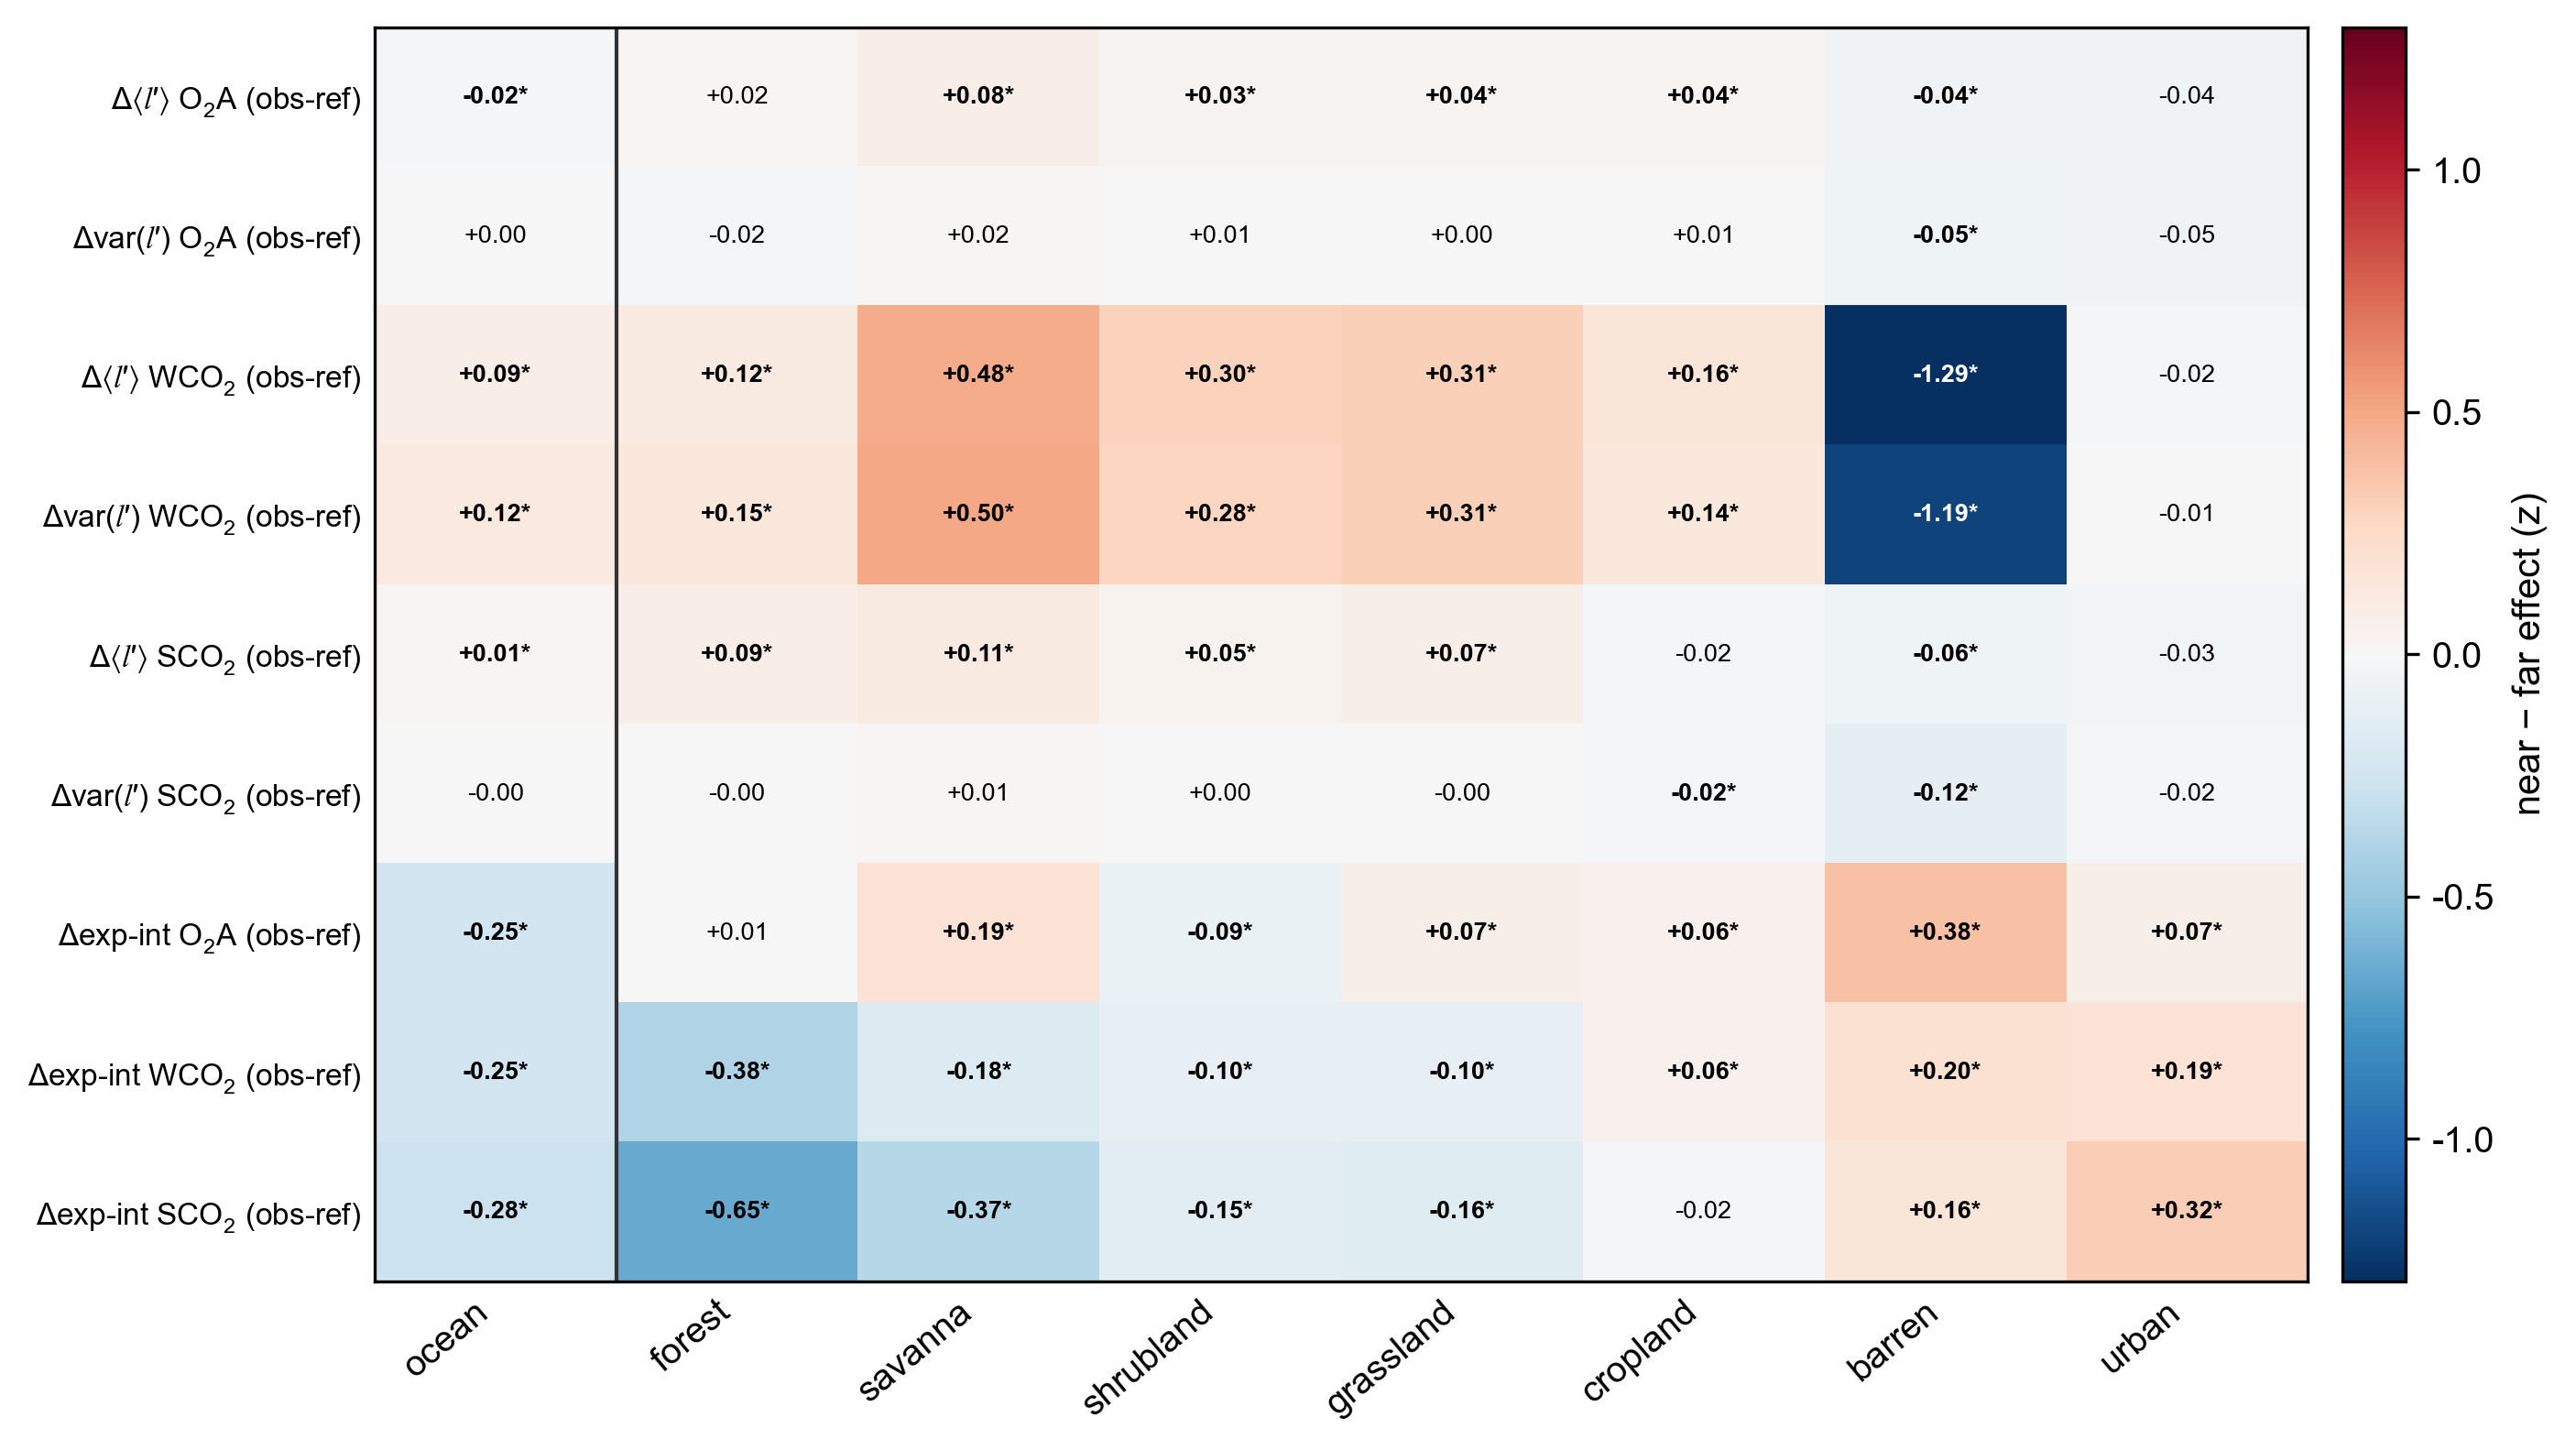
\includegraphics[width=\textwidth]{figures/fig04_landclass_effect_heatmap.png}
\caption{Surface-stratified near-cloud spectral response of effect size (Eq. \ref{eq:effect-size}; near-cloud 0–5 km minus far-cloud 20–50 km, in far-field standard deviations) of the reference-corrected path-length features for ocean and for each MCD12C1 land-cover class. Quality-flag-0, snow-free soundings; per-sounding references use the surface-specific clear-sky radii of the production targets (ocean beyond 5 km, land beyond 15 km); asterisks mark effects exceeding their analytic 95 \% confidence interval. ⟨$l′$⟩ and var($l'$) are the fitted mean and variance of the relative photon path (the cumulants k1, k2 of Sect. 3.2). Reference and quality-flag sensitivity variants: Appendix B.}
\label{fig:land_type_features}
\end{figure}




\begin{figure}[t]
\centering
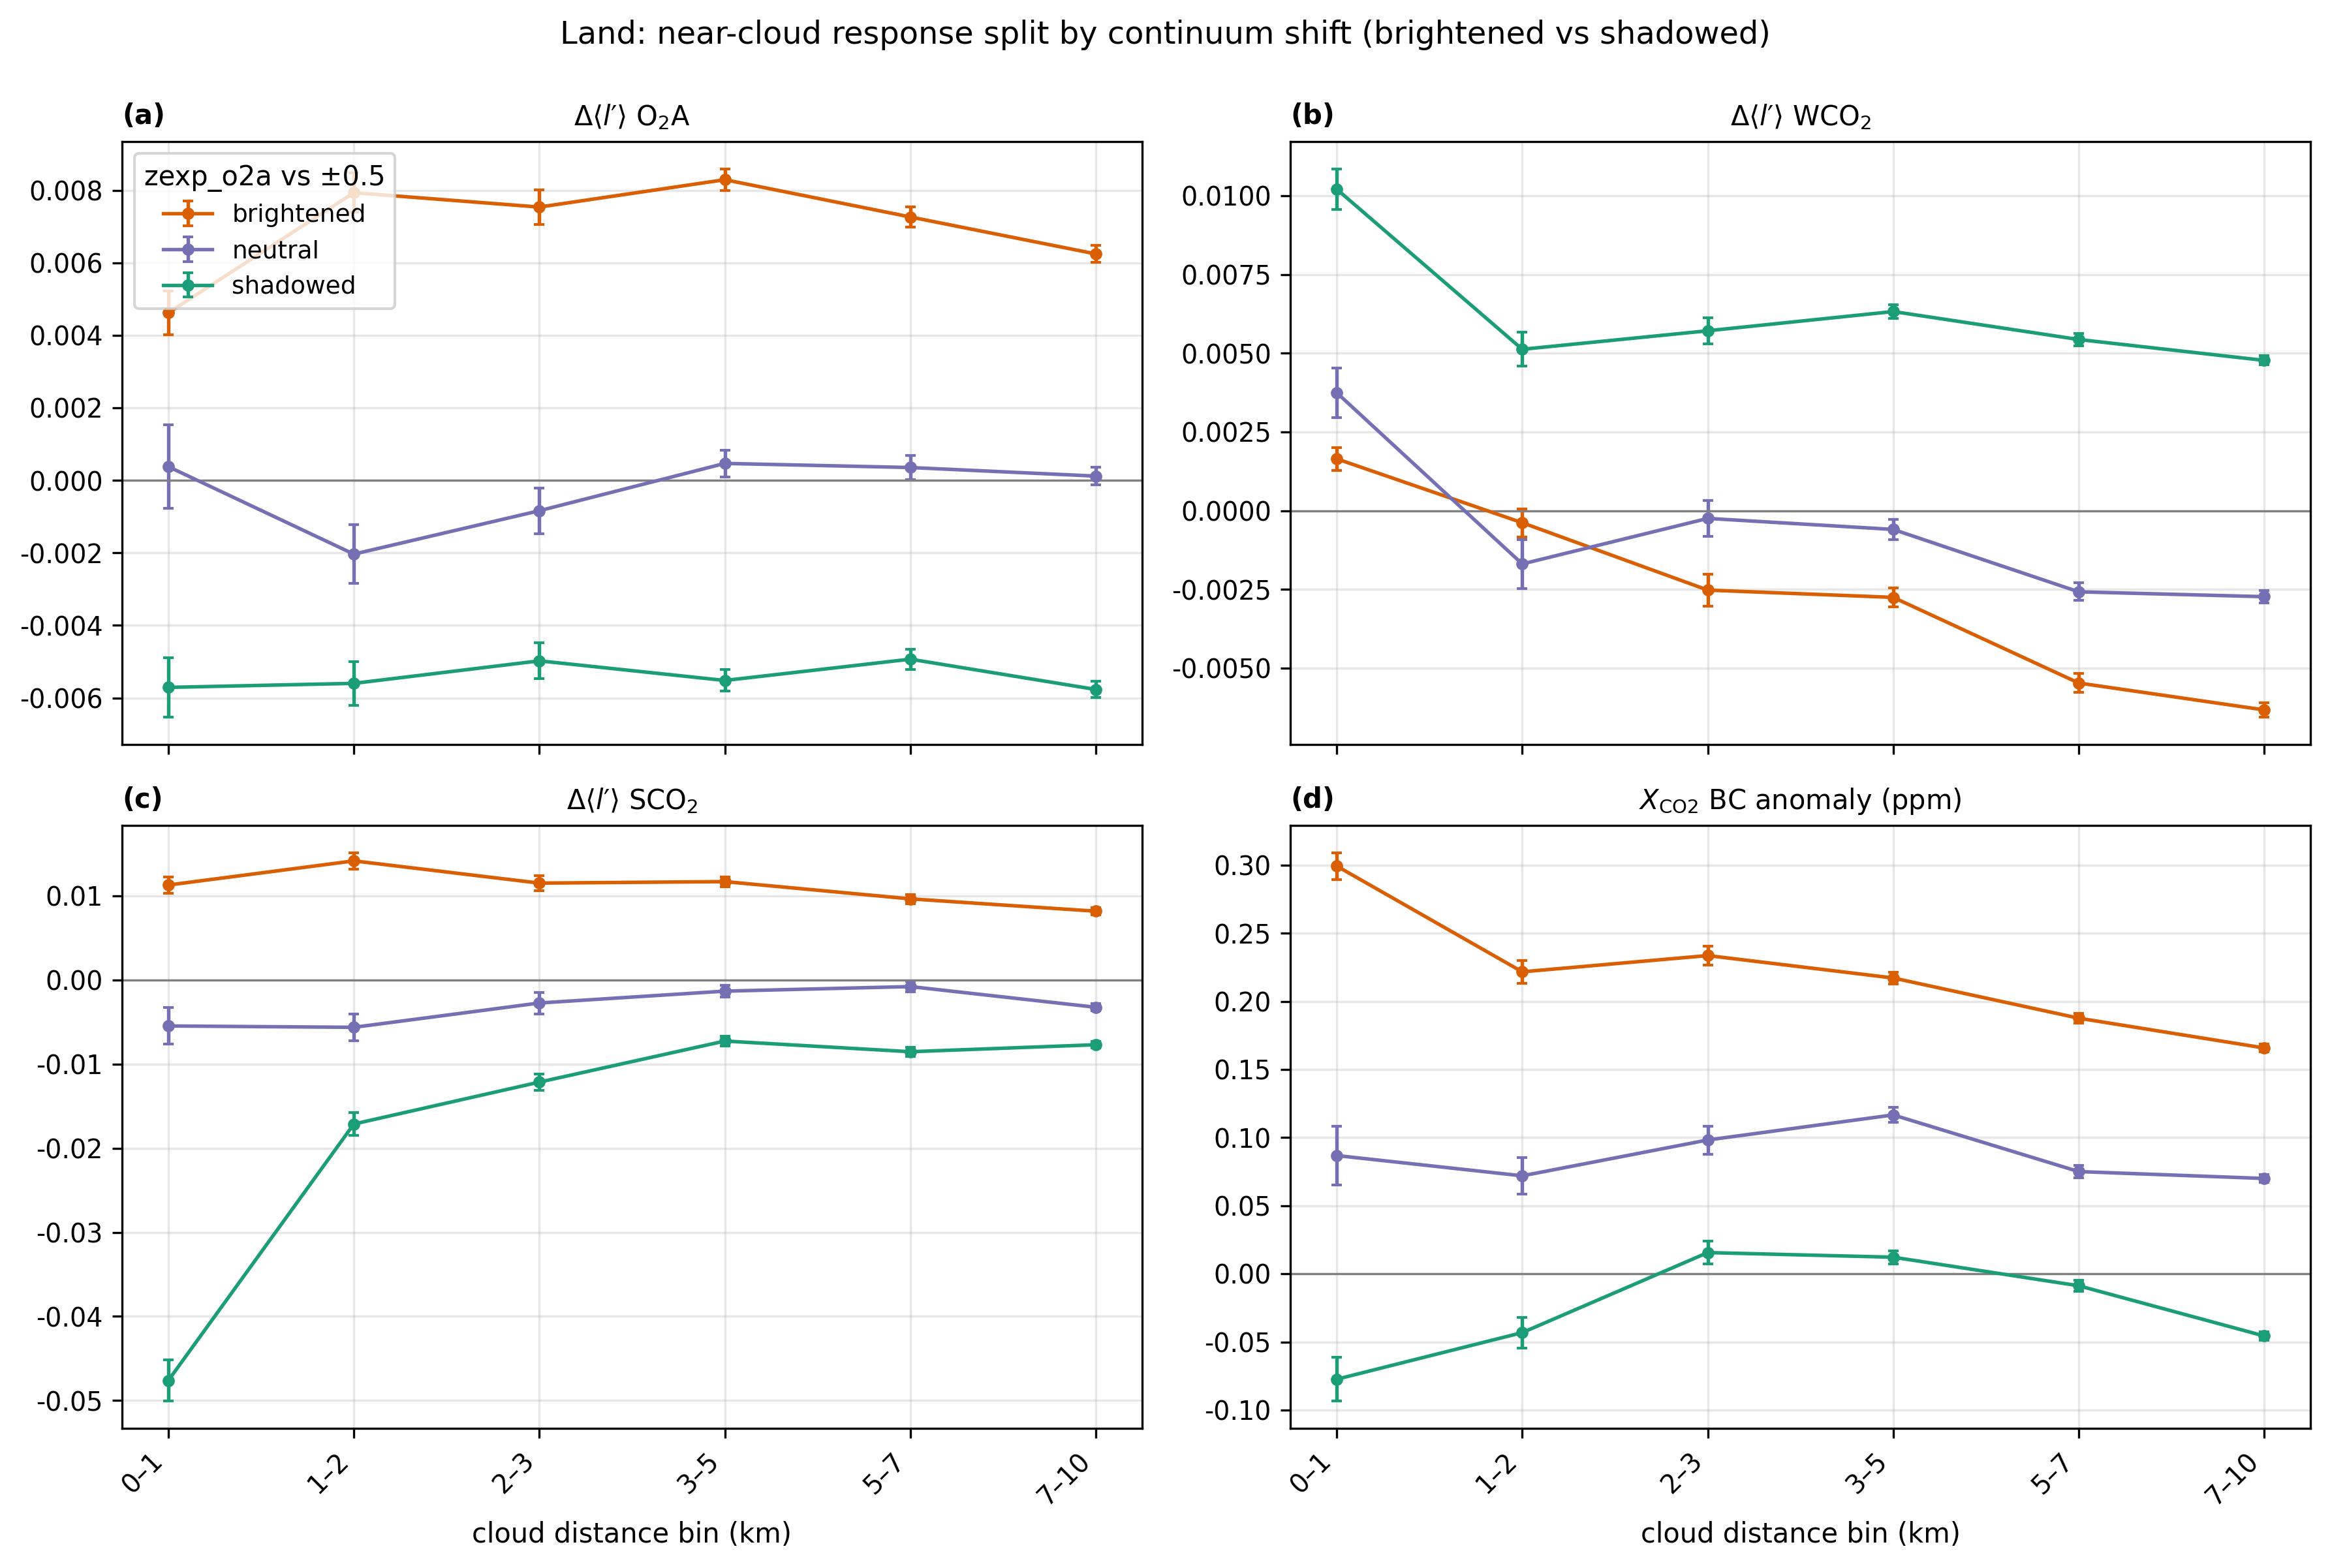
\includegraphics[width=0.8\textwidth]{figures/fig05_shadow_brightening_land.png}
\caption{Shadowing versus brightening. Near-cloud land footprints split by the sign of the \ce{O2}A continuum-reflectance departure from the clear-sky reference (exp-intercept low: cloud shadowing; high: side illumination/brightening), with each branch's \xco anomaly and band-resolved $\Delta$ ⟨$l′$⟩ response. (A single-overpass illustration against Aqua-MODIS true-colour imagery: Appendix G, Fig. G1.)}
\label{fig:shadow-brightening}
\end{figure}




\FloatBarrier

\subsection{Model comparison and feature attribution}
\label{sec:result-model_comp}


The trained \emph{Ridge}, \emph{XGBoost}, and \emph{DE} models with structures and training details in Sect.~\ref{sec:methods-models,sec:method-daataset-split} are compared for their performance over withheld test data and corrected real OCO-2 data. We use ocean and land footprints from the training set to train separate models for ocean and land for all structures. Each model has $5$ members, which are trained on different folds of data (Fig.~\ref{fig:5fold_illustration}). Table~\ref{tab:cv-model-comparison} shows the performance of three models on the same held-out test data. The \emph{DE} has the lowest $RMSE$ and highest $R^2$ when comparing the predicted and true $\Delta$\xcobc, which is better than the \emph{XGBoost} and \emph{Ridge} baselines.


In addition to the $5$ folds held-out test data, we also compare their performance on corrected \xco, which is calculated by
%
\begin{equation}
  \mathrm{X_{CO2}^{model}} = \mathrm{X_{CO2}^{B11}} - \Delta \mathrm{X_{CO2}^{predicted}},
  \label{eq:xco2_corr}
\end{equation}
%
which $\Delta \mathrm{X_{CO2}^{predicted}}$ is predicted \xco anomaly, and $\mathrm{X_{CO2}^{model}}$ is the corrected \xco from different models. The \xcobc, $\mathrm{X_{CO2}^{Ridge}}$, $\mathrm{X_{CO2}^{XGBoost}}$, and $\mathrm{X_{CO2}^{DE}}$ are compared with TCCON measurements following the evaluation method described in Sect.~{sec:method-eval}. Similar to the results of $5$ folds held-out test data, the \emph{DE} model leads at every slice, and the model performance difference is larger in the near-cloud land tail (Fig.~\ref{fig:model_baseline_ablation}a). Though the difference is smaller in the near-cloud ocean tail, the \emph{DE} model still performs better if we consider both the near-cloud ocean tail and QF1 footprints. 

The same ordering holds on the withheld date-blocked folds of the anomaly target (Appendix~\ref{app:model_compare}, Fig.~\ref{fig:model_cv_compare}). The agreement between internal held-out and the independent validations means neither the target construction nor the TCCON chain is driving the selection. Though the fold metrics understate the gap, since the \emph{XGBOOSt} model trails the \emph{DE} model by only ~0.02–0.04 ppm in fold RMSE but by 0.25 ppm on the near-cloud land (≤15 km) TCCON tail. As a result, the \emph{DE} model is used in the later analysis.


After testing the performance over withheld test data and corrected real OCO-2 data, we are interested in the contribution of the feature groups and individual features. We first test removing (1) retrieval-state feature (\xcoraw − \xcoprior), (2) spectral path-length features, and (3) contamination features (See detailed features in Table~\ref{tab:training-config}). As shown in Fig.~\ref{fig:model_baseline_ablation}b, dropping the spectral or contamination groups is TCCON-neutral, whereas removing the retrieval-state departure \xcoraw − \xcoprior) costs 0.8–1.2 ppm. Although using "\xcoraw − \xcoprior" as a feature is similar to looking for an answer of $\Delta$ \xcobc, the $R^2$ between "\xcoraw − \xcoprior" and $\Delta$ \xcobc is only 0.323 for ocean and 0.191 for land. In other words, "\xcoraw − \xcoprior" carries the most abundant cloud-induced \xco bias information, but does not directly reflect the $\Delta$ \xcobc. Even "\xcoraw − \xcoprior" is the most important feature compared to spectral path-length and contamination feature groups, dropping "\xcoraw − \xcoprior" with either spectral path-length or contamination feature groups can degrade the $\Delta \mathrm{RMSE}$ more than not using "\xcoraw − \xcoprior" itself. In particular, dropping "\xcoraw − \xcoprior" with spectral-fitting features shows the largest $\Delta \mathrm{RMSE}$ increase for pooled, near-cloud land and near-cloud ocean tests.


Although the spectral path-length group seems to contribute less than "\xcoraw − \xcoprior" alone, its value lies in three roles "\xcoraw − \xcoprior" cannot fill. First, it indicates the mechanism of cloud-induced bias. The sign rule and shadow/brightening branches of Sect.~\ref{sec:result-spec_anal} establish that the corrected signal is a photon path-length effect, which is something the retrieval-state channel exploits but cannot demonstrate. Second, the spectral path-length group increases the safety of over-correction. The band-resolved fingerprint of Sect.~\ref{sec:result-plume} bounds what the correction may remove. The channel attribution shows the full model removes 55 \% (40–63 \%) of plume-free local clear-sky spread, the no-spectral variant removes 54 \% (the cumulants contribute none of the smoothing essentially), and the no-retrieval-state variant removes 29 \%. The local smoothing flows through the retrieval-state channel while the spectral channel supplies the plume-versus-cloud discriminator. Third, this feature group provides the robustness of imager-independent correction. The cloud-proximity sensitivity of the spectra, including below the MODIS resolution floor (Supplement S4), is what makes imager-free deployment and cross-sensor transfer (Sect.~\ref{sec:disc-img-free}, Appendix H) conceivable. In short, the spectral path-length features establish what the bias is and bound what the correction may touch, while the retrieval-state feature is the operationally sufficient predictor of it.






\begin{figure}[t]
\centering
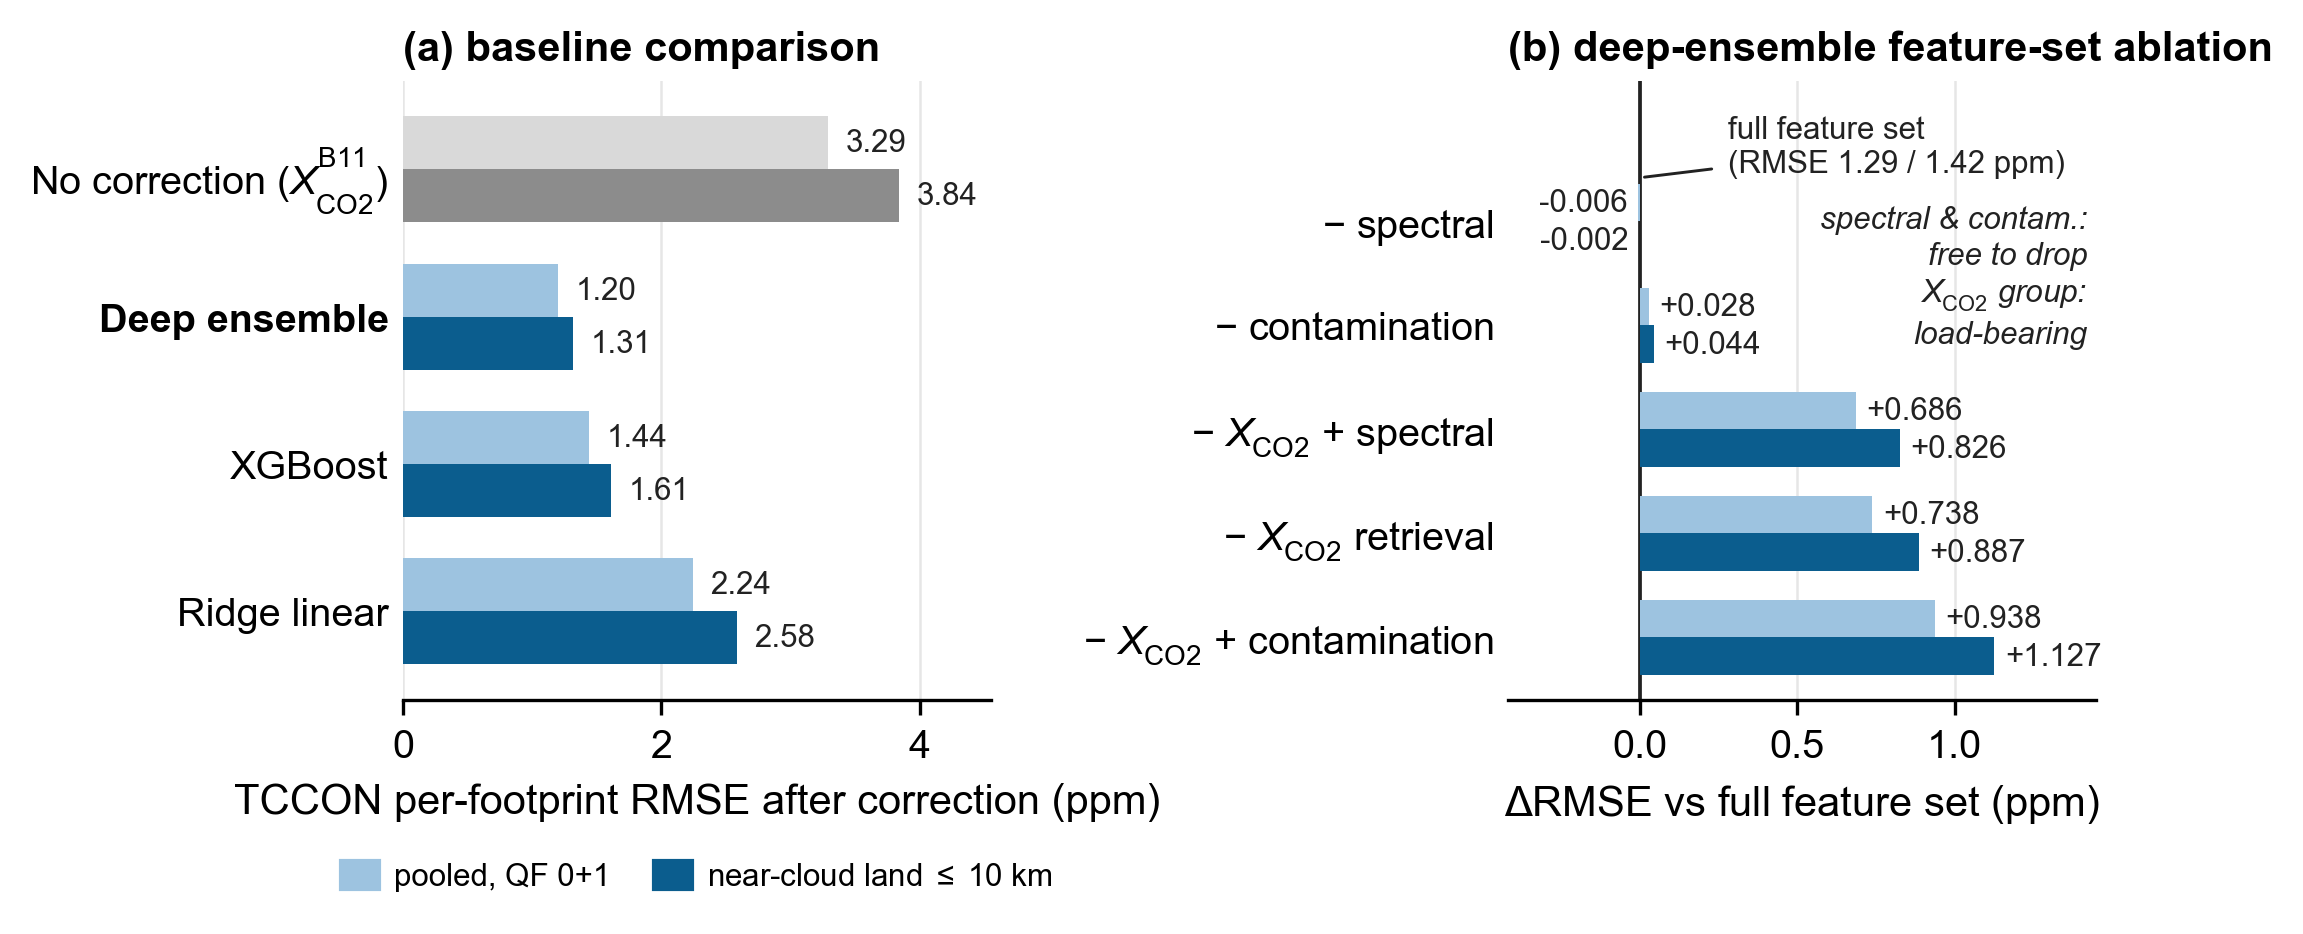
\includegraphics[width=0.8\textwidth]{figures/fig06_baseline_ablation.png}
\caption{Model and feature-set comparison under one protocol (identical features, date-blocked folds, and TCCON chain; AK-harmonised, r = 100 km / ±60 min). (a) TCCON per-footprint RMSE after correction, pooled over all quality flags (light, n = 105,683) and for the near-cloud land subset (≤ 10 km, dark, n = 75,157); the uncorrected product is shown for reference. (b) Feature-group ablation of the deep ensemble: $\Delta$RMSE relative to the full feature set.}
\label{fig:model_baseline_ablation}
\end{figure}



We then evaluate the permutation importance of each variable in the predictors by randomly shuffling each variable to see the increase in $\Delta \mathrm{RMSE}$ for the \emph{DE} model. Same as the results in Fig.~\ref{fig:model_baseline_ablation}b, the "\xcoraw − \xcoprior" plays the most essential role in the bias prediction for both the ocean and land models. The "$\Delta \mathrm{P}$/$\mathrm{P_{surface}^{prior}}$" shows as the second most important variable for both surfaces. Among the spectral path-length features, "var($l'$) of W\ce{CO2}" has the strongest response for the ocean model and the second strongest for the land model. The "$\exp$(\ce{O2}A intercept)" is the most important spectral path-length feature for the land model. The PC1 and PC2 of \ce{CO2} profile EOFs are also crucial for the prediction. Since cloud-bias information can be distributed across several variables in different ways, permuting individual variables may not capture the true importance of each feature. However, this analysis still helps us understand the potential importance of the features.




\begin{figure}[t]
\centering
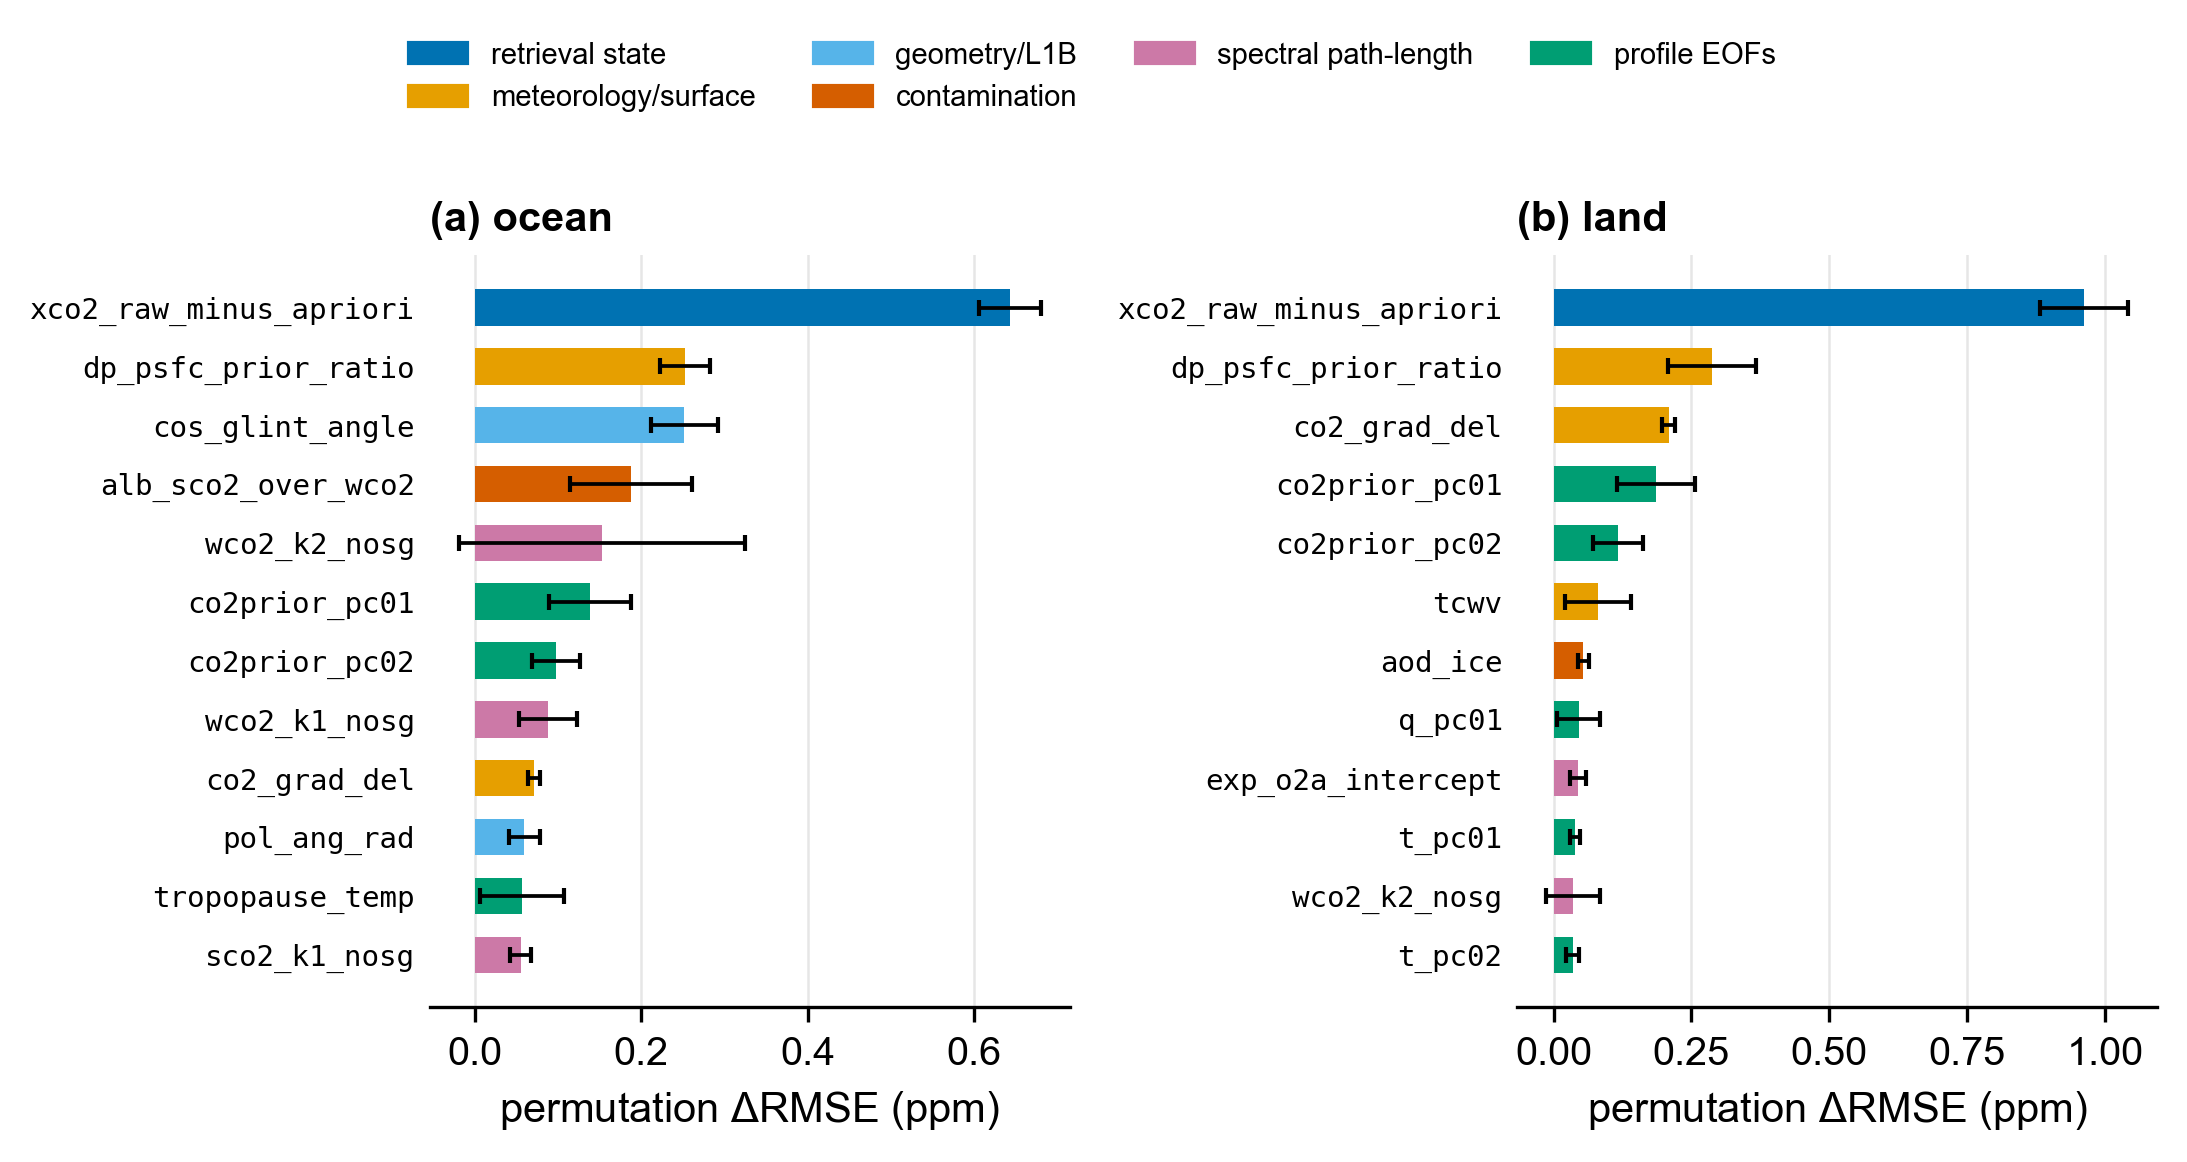
\includegraphics[width=0.8\textwidth]{figures/fig07_feature_importance.png}
\caption{Per-feature permutation importance of the production deep ensemble: increase in held-out fold RMSE when one feature is permuted (median over the five date-blocked folds; whiskers, fold standard deviation), for the twelve highest-ranked features over (a) ocean and (b) land. Bar color gives the predictor group of each feature, with feature definitions in Table~\ref{tab:predictor-inventory}. Groups are permuted jointly in the group-level attribution (Fig.~\ref{fig:model_baseline_ablation}b), which is the appropriate quantity under feature collinearity.}
\label{fig:DE_feature_importance}
\end{figure}




% Generated by manuscript/scripts/make_manuscript_tables.py — do not hand-edit.
% Requires booktabs. Define in the preamble:
%   \newcommand{\xcobc}{$X_{\mathrm{CO2}}^{\mathrm{bc}}$}
%   \newcommand{\xcoraw}{$X_{\mathrm{CO2}}^{\mathrm{raw}}$}
\begin{table}[htbp]
\centering
\caption{Footprint RMSE against AK-harmonized TCCON (ppm; 100\,km / $\pm$60\,min, 75 station-days) before (\xcobc) and after correction by the deep ensemble (DE), XGBoost (XGB), and ridge regression (Ridge). All models share the same footprints and before-column; the best corrected value per slice is in bold. QF is the operational \texttt{xco2\_quality\_flag}; cloud-distance slices split each surface at its production target radius (ocean 5\,km, land 15\,km; Sect.~3.1) and use the pre-drift cases where the Aqua-MODIS collocation is reliable.}
\label{tab:model-comparison}
\small
\begin{tabular}{lrrrrr}
\specialrule{1.2pt}{0pt}{2pt}
Slice & $n$ & Before & DE & XGB & Ridge \\
\midrule
Pooled, QF 0+1 & 105\,683 & 3.29 & \textbf{1.22} & 1.43 & 2.27 \\
Pooled, QF$\,$=$\,$0 & 56\,085 & 1.01 & \textbf{0.83} & 0.87 & 0.92 \\
Pooled, QF$\,$=$\,$1 & 49\,598 & 4.68 & \textbf{1.54} & 1.88 & 3.16 \\
Ocean & 6\,249 & 1.27 & \textbf{0.98} & 1.11 & 1.16 \\
Ocean, QF$\,$=$\,$1 & 1\,578 & 1.76 & \textbf{1.25} & 1.47 & 1.56 \\
Ocean $\leq$5\,km & 2\,645 & 1.54 & \textbf{1.12} & 1.24 & 1.26 \\
Ocean $\leq$5\,km, QF$\,$=$\,$1 & 1\,080 & 1.92 & \textbf{1.29} & 1.46 & 1.52 \\
Ocean $\geq$5\,km & 3\,604 & 1.02 & \textbf{0.86} & 1.01 & 1.08 \\
Land & 99\,434 & 3.38 & \textbf{1.23} & 1.45 & 2.32 \\
Land, QF$\,$=$\,$1 & 48\,020 & 4.75 & \textbf{1.55} & 1.89 & 3.20 \\
Land $\leq$15\,km & 81\,347 & 3.71 & \textbf{1.31} & 1.56 & 2.52 \\
Land $\leq$15\,km, QF$\,$=$\,$1 & 44\,107 & 4.94 & \textbf{1.59} & 1.94 & 3.32 \\
Land $\geq$15\,km & 18\,087 & 0.95 & \textbf{0.79} & 0.85 & 0.98 \\
\specialrule{1.2pt}{2pt}{0pt}
\end{tabular}
\end{table}






% Generated by manuscript/scripts/make_manuscript_tables.py — do not hand-edit.
% Requires booktabs. Define in the preamble:
%   \newcommand{\xcobc}{$X_{\mathrm{CO2}}^{\mathrm{bc}}$}
%   \newcommand{\xcoraw}{$X_{\mathrm{CO2}}^{\mathrm{raw}}$}
\begin{table}[htbp]
\centering
\caption{Feature-group ablation of the mix deep ensemble on TCCON (fp-RMSE, ppm; AK-harmonized reference, 100\,km / $\pm$60\,min). Each variant is retrained from scratch with one feature group removed, using the identical architecture, regularization, and date-blocked folds as the production model (full); all columns share the same footprints and before-column. Dropping the spectral-cumulant or aerosol-contamination groups is TCCON-neutral; the \xcoraw$-$prior departure block carries the correction.}
\label{tab:featureset-ablation}
\small
\begin{tabular}{lrrrrrrr}
\specialrule{1.2pt}{0pt}{2pt}
Slice & Before & full & $-$spec & $-$contam & $-$xco2 & $-$xco2$-$spec & $-$xco2$-$contam \\
\midrule
Pooled, QF 0+1 & 3.29 & \textbf{1.22} & 1.24 & 1.24 & 2.01 & 2.15 & 2.11 \\
Pooled, QF$\,$=$\,$0 & 1.01 & 0.83 & \textbf{0.83} & 0.85 & 1.03 & 0.99 & 1.12 \\
Pooled, QF$\,$=$\,$1 & 4.68 & \textbf{1.54} & 1.58 & 1.58 & 2.72 & 2.96 & 2.84 \\
Ocean & 1.27 & \textbf{0.98} & 1.00 & 0.99 & 1.13 & 1.15 & 1.15 \\
Land & 3.38 & \textbf{1.23} & 1.25 & 1.26 & 2.05 & 2.20 & 2.16 \\
Land, QF$\,$=$\,$1 & 4.75 & \textbf{1.55} & 1.59 & 1.59 & 2.76 & 2.99 & 2.88 \\
Land $\leq$10\,km & 3.84 & \textbf{1.33} & 1.36 & 1.36 & 2.30 & 2.47 & 2.42 \\
Land $\leq$10\,km, QF$\,$=$\,$1 & 5.00 & \textbf{1.60} & 1.64 & 1.63 & 2.88 & 3.14 & 3.01 \\
Land $\geq$10\,km & 1.00 & 0.84 & \textbf{0.83} & 0.90 & 0.91 & 0.97 & 0.98 \\
\specialrule{1.2pt}{2pt}{0pt}
\end{tabular}
\end{table}






\FloatBarrier

\subsection{Independent TCCON validation}
\label{sec:result-tccon_val}


%Use AK-harmonized TCCON as the primary reference and direct TCCON as a
%documented secondary comparison. Report the current production values only
%after regenerating the manuscript table from the frozen tag.

%The paragraph order should be:

1. one-sentence recap of the sample and coincidence criteria, citing
   Sect. 3.5;
2. mean absolute bias and footprint RMSE;
3. number of improved station-days;
4. Wilcoxon and site-clustered bootstrap results;
5. radius/window and QF0/QF1 sensitivity;
6. high-latitude and worsening cases.

Keep direct-reference results nearby but do not let the dual-reference
explanation obscure the AK-harmonized primary result.


After understanding the general performance of the \emph{DE} model in Sect.~\ref{sec:result-model_comp}, we then evaluate its correction capability compared to TCCON observations in detail. Again, all TCCON \xco are corrected following the description in Sect.~\ref{sec:method-eval-obs-xco2} to consider the difference in averaging kernels and prior profiles. The collocation search radius between the TCCON stations and the OCO-2 soundings is set to $100$~km, and the temporal search window to $\pm1$~h around the OCO-2 overpass. Note that these 75 station-days for 18 sites from December 2014 to December 2021 are chosen manually, as we want to have more available data for stations near the coastline, and we are unable to run all OCO-2 overpass cases.


Across all 75 station-days, the station-day mean absolute bias ($|$bias$|$) falls from 1.26$\pm$1.33 to 0.82$\pm$0.60 ppm and the per-footprint RMSE from 2.67 to 1.20 ppm (Fig.~\ref{fig:tccon_dumbbel}). The per-footprint RMSE improves in 71 of the 75 station-days, while the station-day mean bias improves in 46 of 75. The remaining 29 worsen only slightly, median $+0.28$ ppm, mostly from near-zero starting biases. The improvement is significant under a paired Wilcoxon test on station-day $|$bias$|$ (p = 0.0063, n = 75) and under site-clustered bootstrap intervals, with and without the high-latitude TCCON station Ny-Ålesund at 78.93$^\circ$N (Fig.~\ref{fig:tccon_significance_robustness}). The improvement holds at every collocation radius $\times$ window combination (25/50/100 km $\times$ $\pm$30/60/120 min), and it is largest at a tighter 50 km $\times$ $\pm$30 min window. This is expected, given that the correction is a spatially localized process. However, we use a larger search window to obtain more statistics and follow the $\pm1$~h window as in \citet{das2025oco2_v111_tccon_ggg2020}.

Additionally, we analyze QF=0 and QF=1 footprints separately (Fig.~\ref{app-fig:qf01_DE_eval}) and see that the $|$bias$|$ significantly decreases for QF=1 from 1.57$\pm$1.43 to 0.89$\pm$0.62, with the footprint RMSE reduced from 3.19 to 1.31. The $|$bias$|$ and footprint RMSE also improve for QF=0 but with smaller magnitudes. This is expected, as footprints with QF=0 have better retrieval quality and could be less influenced by clouds. We also see that the correction is larger when the station-mean nearest-cloud distance of OCO-2 footprints is small, confirming that our correction works in the right direction.

For all TCCON stations we used, Ny-Ålesund is the only station in our comparison poleward of 60$^\circ$ latitude, and high-latitude scenes are correspondingly rare in the training population. Only 5.3\,\% of the 17.8 million training
footprints lie poleward of $|60^\circ|$ (936,178) and 2.3 \% poleward of $|70^\circ|$ (411,649). Nevertheless, the ten Ny-Ålesund station-days receive the strongest corrections in the network. The station-day mean $|$bias$|$ falls from 2.18 to 1.31~ppm and the per-footprint RMSE from 4.74 to 1.95~ppm, both roughly twice the network-average improvement. The largest single correction of the comparison (from $-8.20$ to $-0.86$~ppm on 17 June 2017) occurs here. This is also why excluding
Ny-Ålesund reduces the magnitude of all three aggregate improvements in Fig.~\ref{fig:tccon_significance_robustness}a while their significance is retained ($p \le 0.016$). The headline result is not driven by this single site, but the site benefits from the correction more than any
other. At the same time, the corrected Ny-Ålesund residuals remain the largest in the network and are sign-consistent (positive in 7 of 10 station-days, up to $+2.9$~ppm), so a systematic high-latitude bias
survives the correction. We attribute this remaining bias to the thin training support poleward of 60$^\circ$ together with the extreme observation geometry (high solar zenith angle, seasonal snow and ice), and we regard the high-latitude regime as the part of the domain where the correction is least constrained. Additional high-latitude references (e.g., Sodankylä, East Trout Lake, Eureka) would be needed to validate it independently, and we return to this limit in Sect.~\ref{sec:limitation}.


The worsening cases are informative about the limits of the anomaly formulation rather than about the model fit. The bright-surface stratum (\ce{O2}A-band albedo $> 0.4$; 12{,}037 footprints, 11.4\,\% of the TCCON comparison set) shows the largest post-correction residual (1.55~ppm) and a worsened-footprint fraction of 0.50. This is not a prediction failure: on genuinely held-out dates in cross-validation, the model's anomaly skill is independent of albedo (residual RMSE 0.53--0.60~ppm and calibration $\langle z^2\rangle \approx 1.1$ across all albedo deciles), and even at TCCON the correction reduces the bright-surface footprint RMSE from 4.58 to 1.55~ppm. What remains after correction over bright scenes is a bias component that is nearly constant within an overpass. Such a common-mode component cancels in the within-orbit anomaly target by construction, so the model is never trained to remove it; the correction takes out the anomaly part and leaves the common-mode part behind. Because the remaining residual is then uncorrelated with the applied correction, the per-footprint worsened-or-improved count degenerates toward a coin flip (0.50, against 0.19--0.39 elsewhere), while the aggregate error still improves. The bright-surface stratum is therefore under-corrected rather than mis-corrected, in line with the high-AOD stratum, and both point to the same future extension: a complementary term for along-track common-mode bias, which the present per-footprint anomaly correction intentionally does not model.





\begin{figure}[t]
\centering
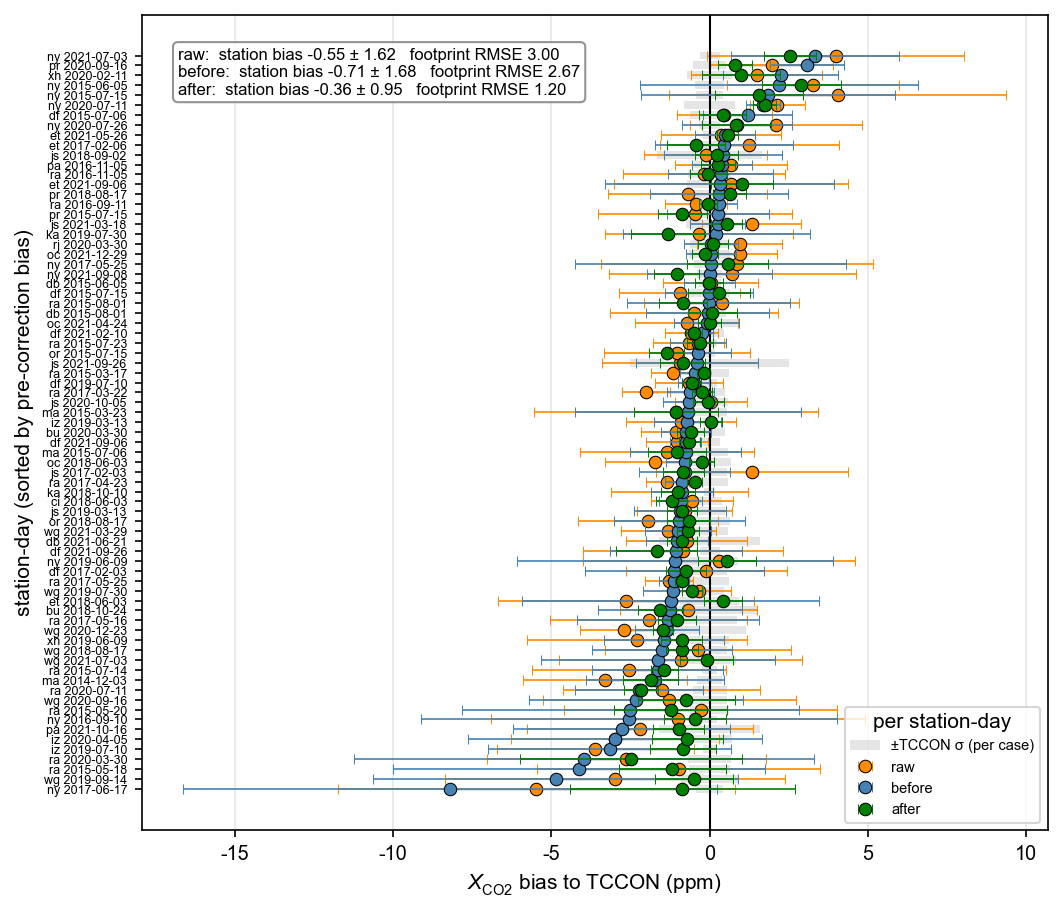
\includegraphics[width=0.8\textwidth]{figures/fig08_tccon_dumbbell.png}
\caption{Independent TCCON validation (AK-harmonised reference; before-vs-after differences are invariant to it): station-day mean bias before and after correction for all 75 station-days (18 sites, 2014–2021; r = 100 km, ±60 min).}
\label{fig:tccon_dumbbel}
\end{figure}



\begin{figure}[t]
\centering
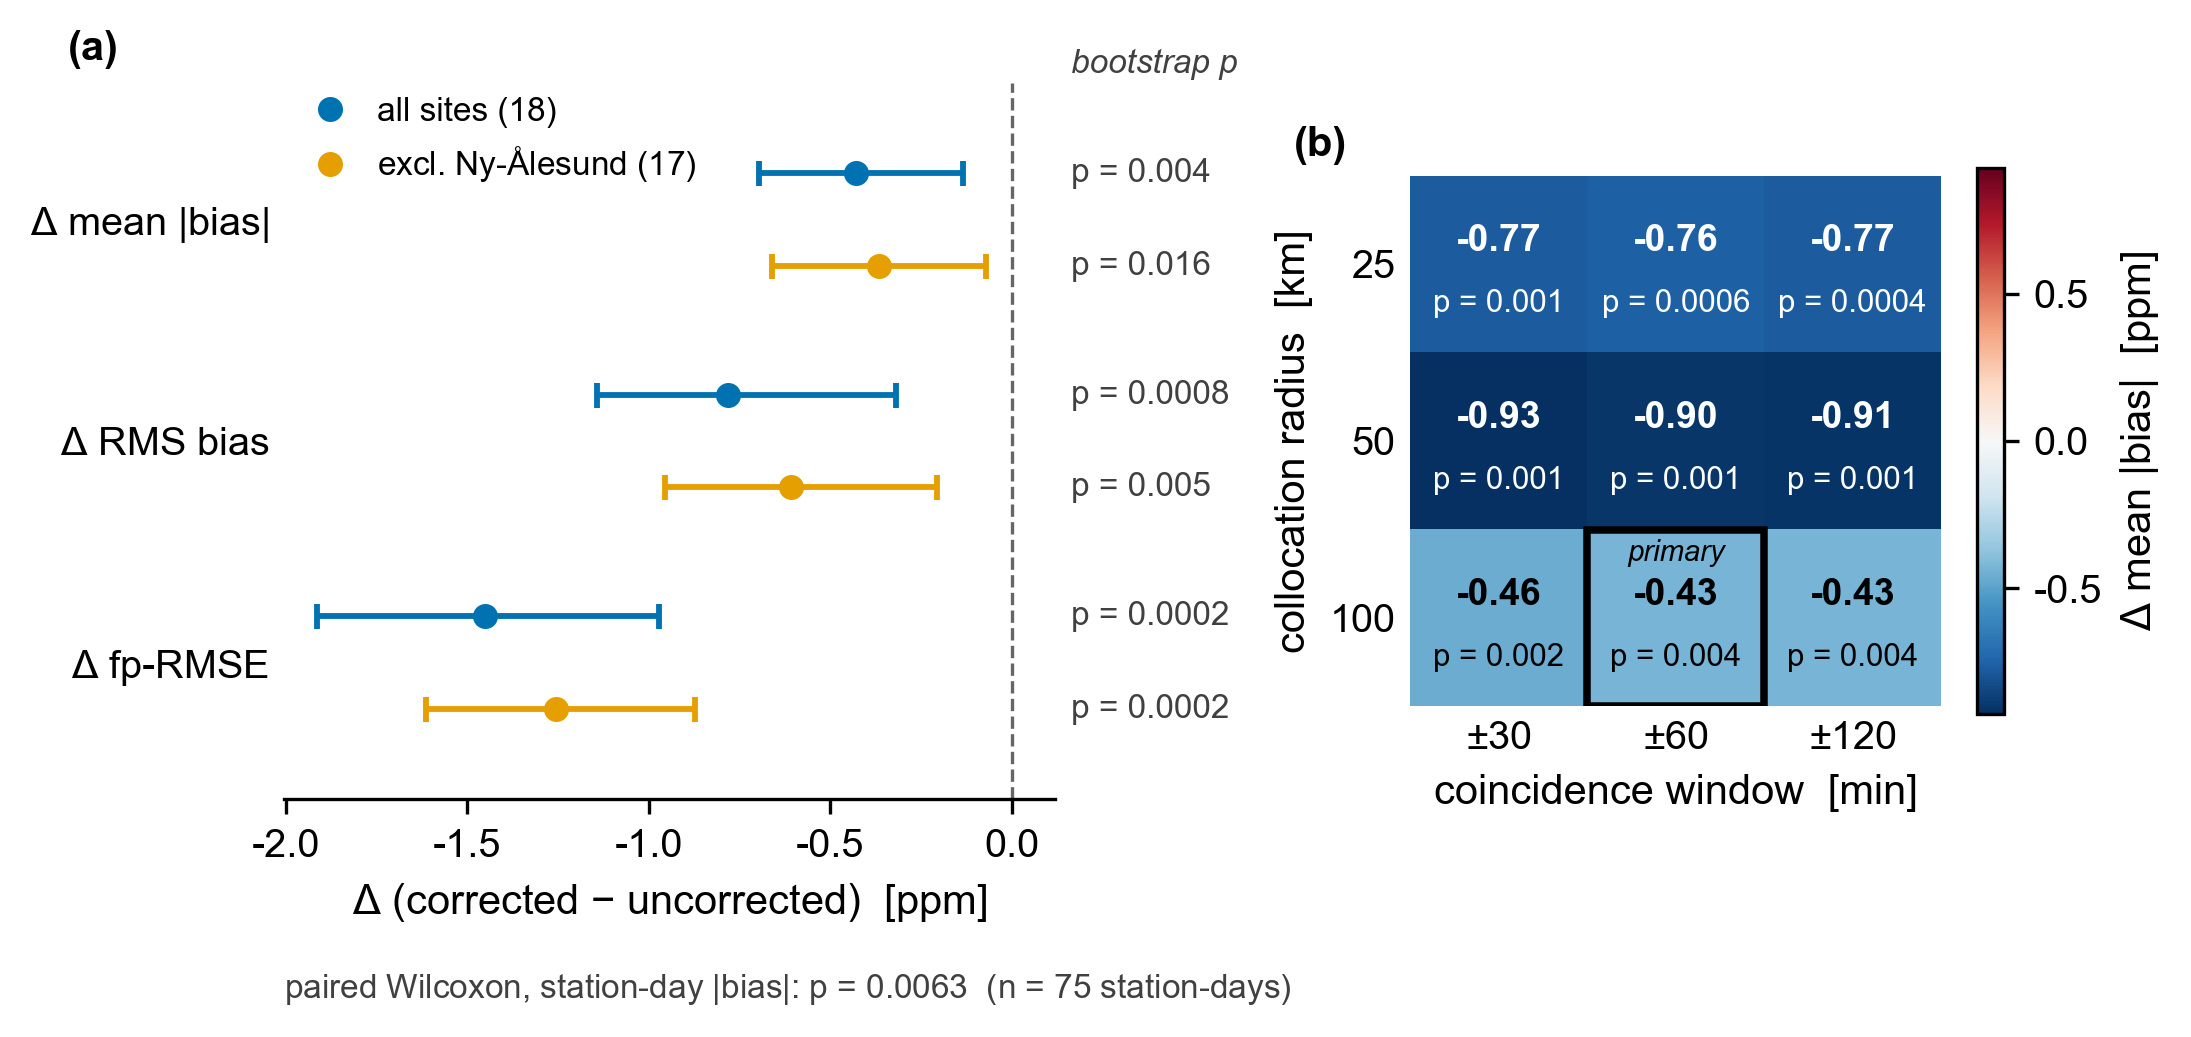
\includegraphics[width=0.8\textwidth]{figures/fig09_significance_robustness.png}
\caption{Significance and robustness of the TCCON validation: site-clustered bootstrap estimates with 95 \% confidence intervals for the change in station-day mean $|$bias$|$, RMS bias, and per-footprint RMSE (all sites and excluding Ny-Ålesund), and the change in mean $|$bias$|$ across collocation radius (25/50/100 km) × window (±30/60/120 min).}
\label{fig:tccon_significance_robustness}
\end{figure}





%% Generated by manuscript/scripts/make_manuscript_tables.py — do not hand-edit.
% Requires booktabs. Define in the preamble:
%   \newcommand{\xcobc}{$X_{\mathrm{CO2}}^{\mathrm{bc}}$}
%   \newcommand{\xcoraw}{$X_{\mathrm{CO2}}^{\mathrm{raw}}$}
\begin{table}[htbp]
\centering
\caption{Station-equal mean absolute bias to AK-harmonized TCCON (ppm): each station's footprint-weighted mean bias is taken in absolute value and averaged with equal station weights (18 stations). Best corrected value per row in bold.}
\label{tab:station-equal-bias}
\small
\begin{tabular}{lrrrr}
\specialrule{1.2pt}{0pt}{2pt}
QF & Before & DE & XGB & Ridge \\
\midrule
QF 0+1 & 0.98 & \textbf{0.73} & 0.74 & 0.83 \\
QF$\,$=$\,$0 & 0.60 & 0.60 & 0.63 & \textbf{0.58} \\
QF$\,$=$\,$1 & 1.36 & 0.82 & \textbf{0.80} & 0.96 \\
\specialrule{1.2pt}{2pt}{0pt}
\end{tabular}
\end{table}






\FloatBarrier

\subsection{Distinguishing correction from smoothing}
\label{sec:result-corr_smooth}


A possible objection to the decrease in footprint RMSE result of Sect.~\ref{sec:result-tccon_val} is that the \emph{DE} model may act as a local low-pass filter. Since the near-cloud bias appears as short-scale structure along the orbit, any procedure that averages neighboring footprints would also collapse the within-overpass scatter, and the station-day comparison might not distinguish the two. To test this possibility directly, we construct a feature-free smoother null and evaluate it with exactly the same footprints, output guards, and AK-harmonized TCCON chain as the production correction.

For footprint $i$, the smoothed product is the orbit-local running mean of the operational product,
%
\begin{equation}
  X^{\mathrm{sm}(W)}_{\mathrm{CO2},i}
  = \frac{1}{\left|\mathcal{N}_i(W)\right|}
    \sum_{j \in \mathcal{N}_i(W)} X^{\mathrm{B11}}_{\mathrm{CO2},j},
  \qquad
  \mathcal{N}_i(W)
  = \left\{\, j \;:\; \left|t_j - t_i\right| \le W \,\right\},
  \label{eq:smoother}
\end{equation}
%
where $t_i$ is the sounding time and $\mathcal{N}_i(W)$ is restricted to the same contiguous along-track segment (a time gap larger than 30~s starts a new segment) and the same surface type as footprint $i$, mirroring the per-surface construction of the model; the footprint itself is included in the mean, as for any symmetric smoother. The implied pseudo-correction is $\mu^{\mathrm{sm}}_i = X^{\mathrm{B11}}_{\mathrm{CO2},i} - X^{\mathrm{sm}(W)}_{\mathrm{CO2},i}$, which replaces the deep-ensemble $\mu_i$ in the evaluation chain. We test half-widths $W = 10$, 30, and 100~s, corresponding to roughly $\pm 67$, $\pm 200$, and $\pm 675$~km along track. The smoother uses no predictor features and no cloud information: it is the strongest form of the ``the correction only smooths'' hypothesis.

The two diagnostics separate cleanly (Fig.~\ref{fig:smoother_null}). On the within-overpass footprint scatter, the smoother is stronger than the \emph{DE} model as expected. The per-case mean scatter falls from 2.23~ppm to 0.66, 0.51, and 0.35~ppm for $W = 10$, 30, and 100~s, compared with 0.78~ppm for the deep ensemble. A running mean minimizes local variance by construction, so on this metric alone the null cannot be rejected. The station-day mean $|$bias$|$ to TCCON, however, is left essentially unmoved by the smoother: 1.26~ppm before correction against 1.24, 1.20, and 1.20~ppm after smoothing, whereas the deep ensemble reduces it to 0.82~ppm. The reason is structural: because the running mean approximately preserves the overpass-mean \xco, it can only redistribute the error among footprints, not remove it, while the deep ensemble shifts the mean itself. We conclude that variance removal alone cannot reproduce the observed bias reduction, and that the validation improvement of Sect.~4.4 reflects a genuine correction of the near-cloud bias rather than local denoising. Figure~\ref{fig:smoother_null} shows the $W = 30$~s arm; the $\pm 10$ and $\pm 100$~s arms behave the same way and are given in Appendix~\ref{app:null-test} (Fig.~\ref{app-fig:smoother_null_full}).




The smoother collapses footprint scatter more strongly than the \emph{DE} model (0.35–0.66 vs 0.78 ppm) yet leaves the TCCON station-day mean $|$bias$|$ essentially unmoved (1.20–1.24 ppm, against 0.82 ppm for the model). In other words, variance removal alone cannot produce the observed bias reduction, and the correction by the \emph{DE} model reduces both observed bias and spread.




\begin{figure}[t]
\centering
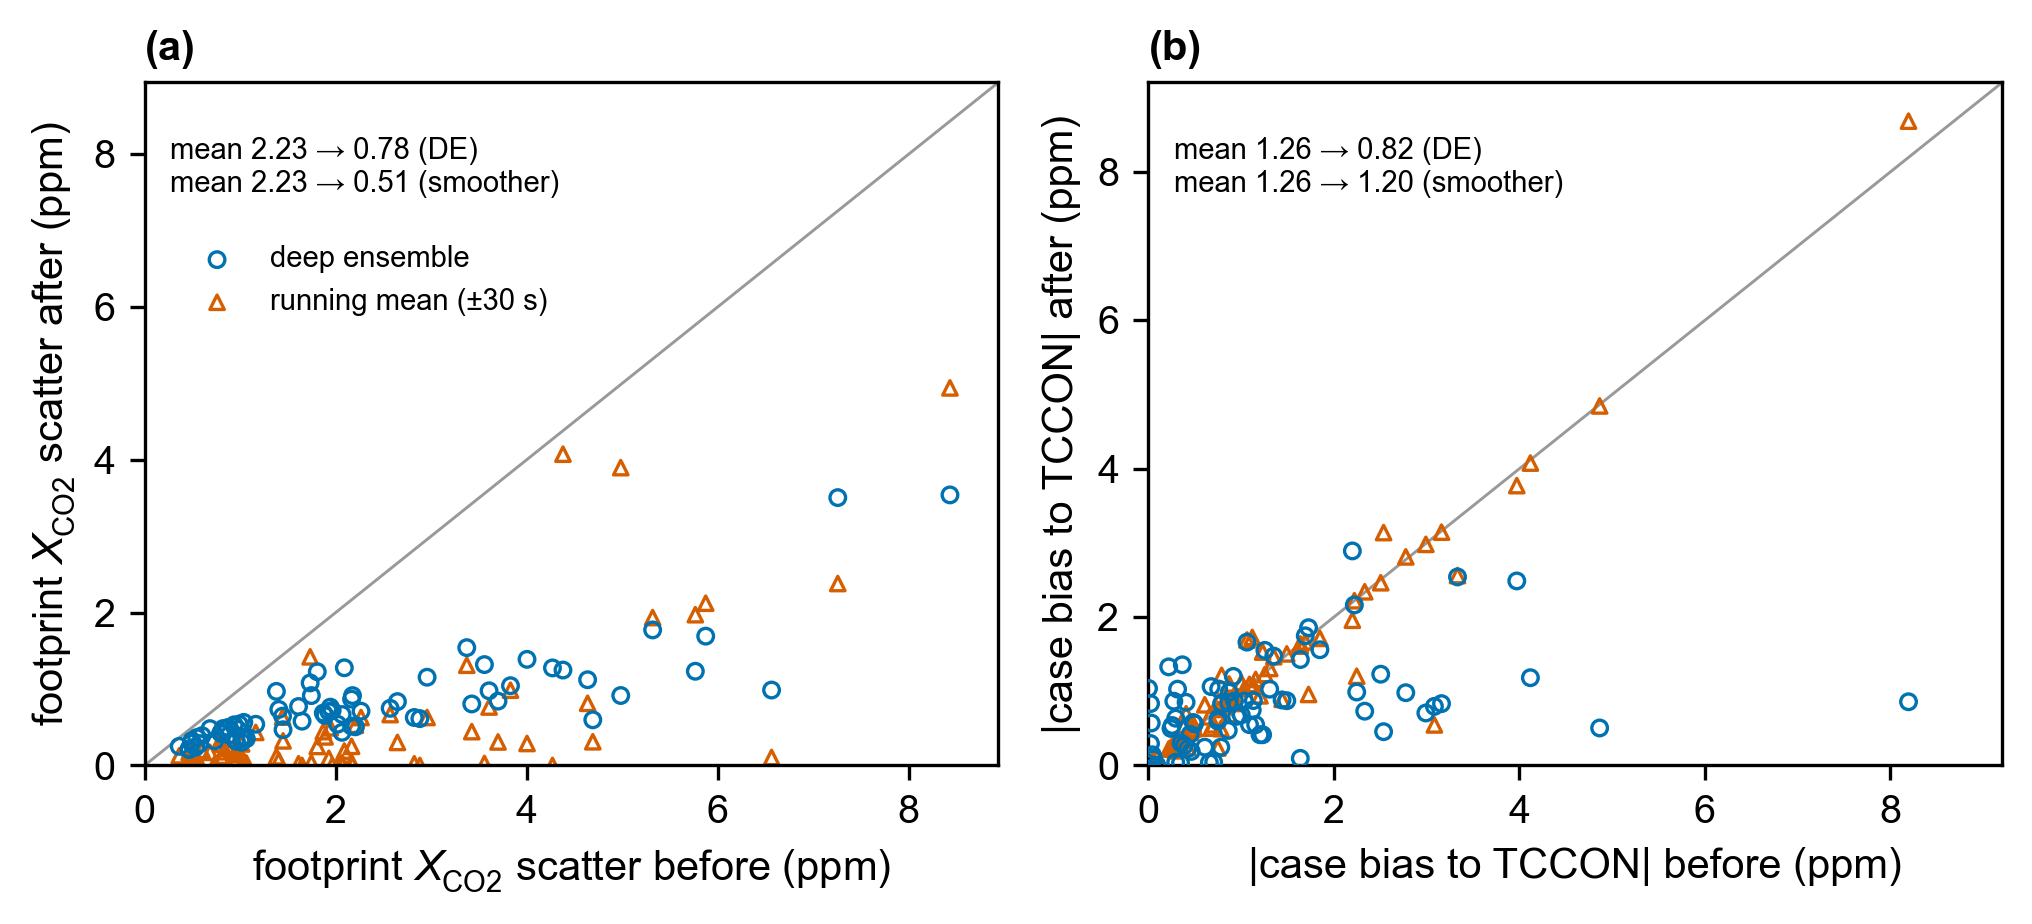
\includegraphics[width=0.8\textwidth]{figures/fig10_smoother_null.png}
\caption{Correction versus smoothing null test. A feature-free orbit-local running-mean smoother (±10/30/100 s half-widths, screened by the same input guards as the production correction) compared with the deep ensemble on footprint scatter (a) and TCCON station-day mean $|$bias$|$ (b).}
\label{fig:smoother_null}
\end{figure}



\FloatBarrier

\subsection{Ocean validation and far-cloud controls}
\label{sec:result-ocean_far_cldl}

Present ATom, shipborne EM27/SUN, and the far-cloud/clear-day cases where the
correction is nearly inert. Treat these as independent corroboration, not as
equivalent in statistical weight to TCCON. State the limited sample and
reference-scale caveats.


After we validate the correction of the \emph{DE} model in Sect.~\ref{sec:result-tccon_val,sec:result-corr_smooth}, we extend our validation to two different in-situ measurements to provide more validation tests over the ocean, considering that all TCCON stations are still over land and only part of them are close to the ocean coastline. We identify 17 ATom and OCO-2 co-located legs and 4 shipborne (MORE-2 and MR21-01) and OCO-2 co-located legs. We construct the pseudo-column \xcoatom from the in-situ airborne \xco measurement for comparison (Sect.~\ref{sec:method-eval-obs-xco2}), and use \xcoship directly as no prior profiles and averaging kernels are available.


Across the 17 ATom legs (14 near-cloud), the near-cloud improvement is a scatter reduction, not an offset shift. The median $|$residual$|$ ($|$\xcooco - \xcoatom$|$) falls from 0.53 to 0.45 ppm and the across-leg spread from ±0.72 to ±0.58 ppm, while the signed mean bias is essentially unchanged (+0.19 → +0.20 ppm, well within the per-leg pseudo-column $\sigma$ of 0.10–0.19 ppm). The far-cloud date (9 October 2017) is a negative control that the correction leaves nearly unchanged (Fig.~\ref{fig:ocean-validation}a, b). Against the shipborne EM27/SUN spectrometers (4 cases, 3 near-cloud), the correction collapses footprint scatter (mean $\sigma$ 0.63 → 0.27 ppm, against a mean ship reference $\sigma$ of 0.29 ppm) without moving the clear-sky control day (22 June 2019). The increase of $|$residual$|$ ($|$\xcooco - \xcoship$|$) absolute offset (all-case mean +0.99 ± 0.70 before, +1.18 ± 0.81 ppm after) could be dominated by reference-scale differences, considering no prior profiles and averaging kernel-harmonization applied  (Fig.~\ref{fig:ocean-validation}c, d). Note that we have limited temporal and spatial overpass samples compared to TCCON validations for ATom and Shipborne measurements comparison. The comparison with ATom in-situ and shipborne EM27/SUN measurements should be treated as independent corroboration, not as equivalent in statistical weight to TCCON.


Figure~\ref{app-fig:atom_far_cld,app-fig:ship_far_cld} illustrate little change in values and distribution for far-cloud footprints for ATom and Ship observation cases. These two negative controls are consistent with the far-cloud behavior in the TCCON comparison itself. In the station-day groups beyond the
production reference radii (ocean $\geq 5$~km, land $\geq 15$~km; Table~\ref{tab:model_comparison}), the pre-correction error is already small, and the correction leaves it slightly improved rather than degraded (footprint RMSE 1.02 $\rightarrow$ 0.86 and 0.95 $\rightarrow$ 0.79~ppm, respectively; see also the cloud-distance dependence in Fig.~\ref{app-fig:qf01_DE_eval}), so the near-inert far-cloud response over the ocean is not a small-sample artifact.



\begin{figure}[t]
\centering
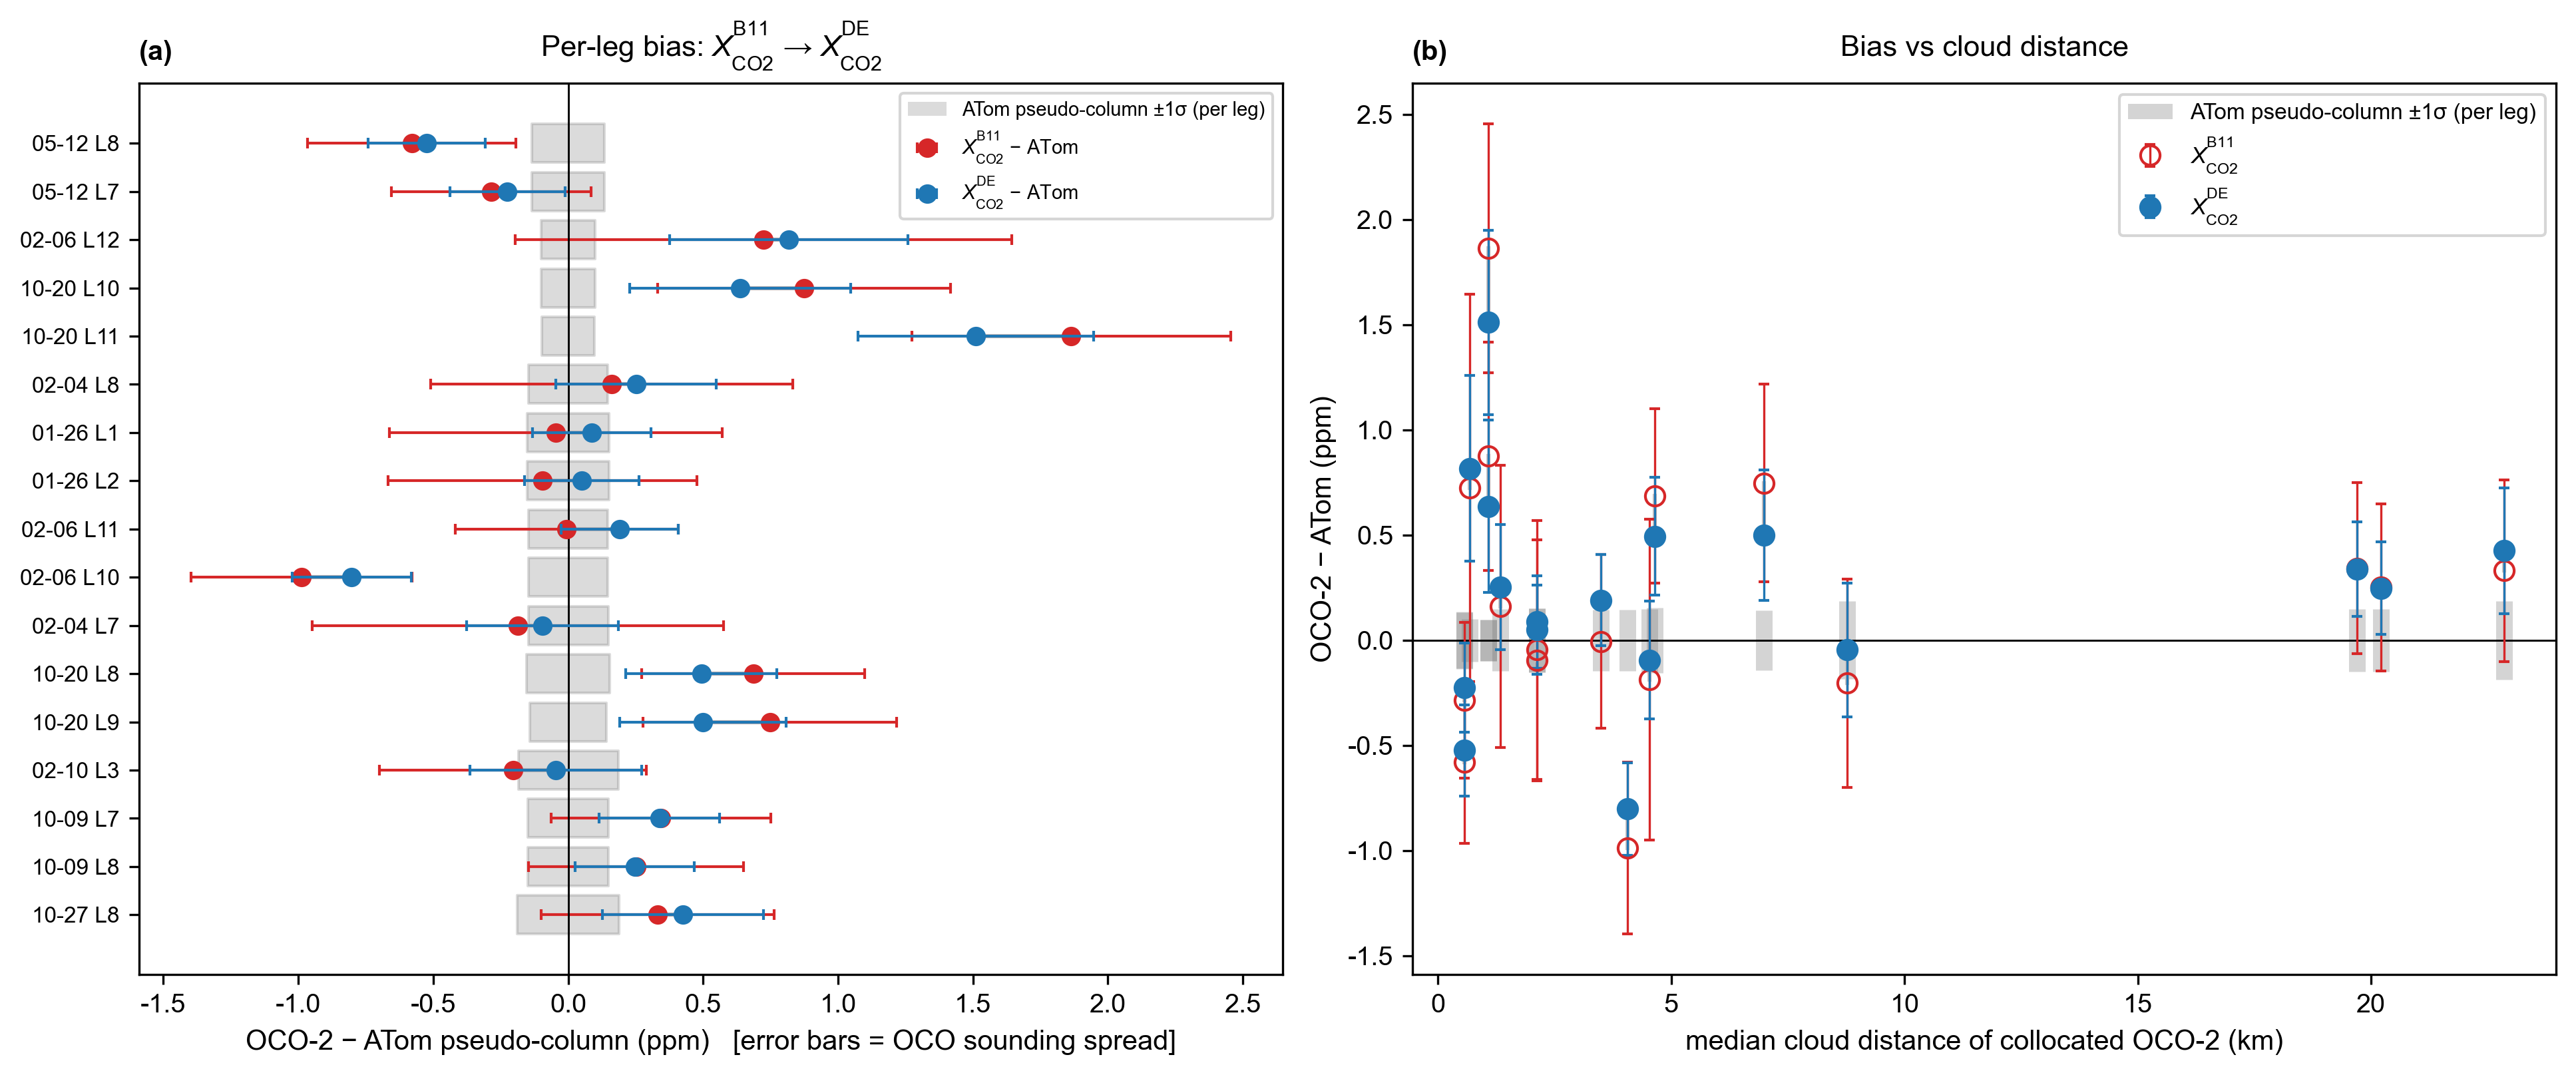
\includegraphics[width=0.95\textwidth]{figures/fig11a_atom_summary.png}\\[4pt]
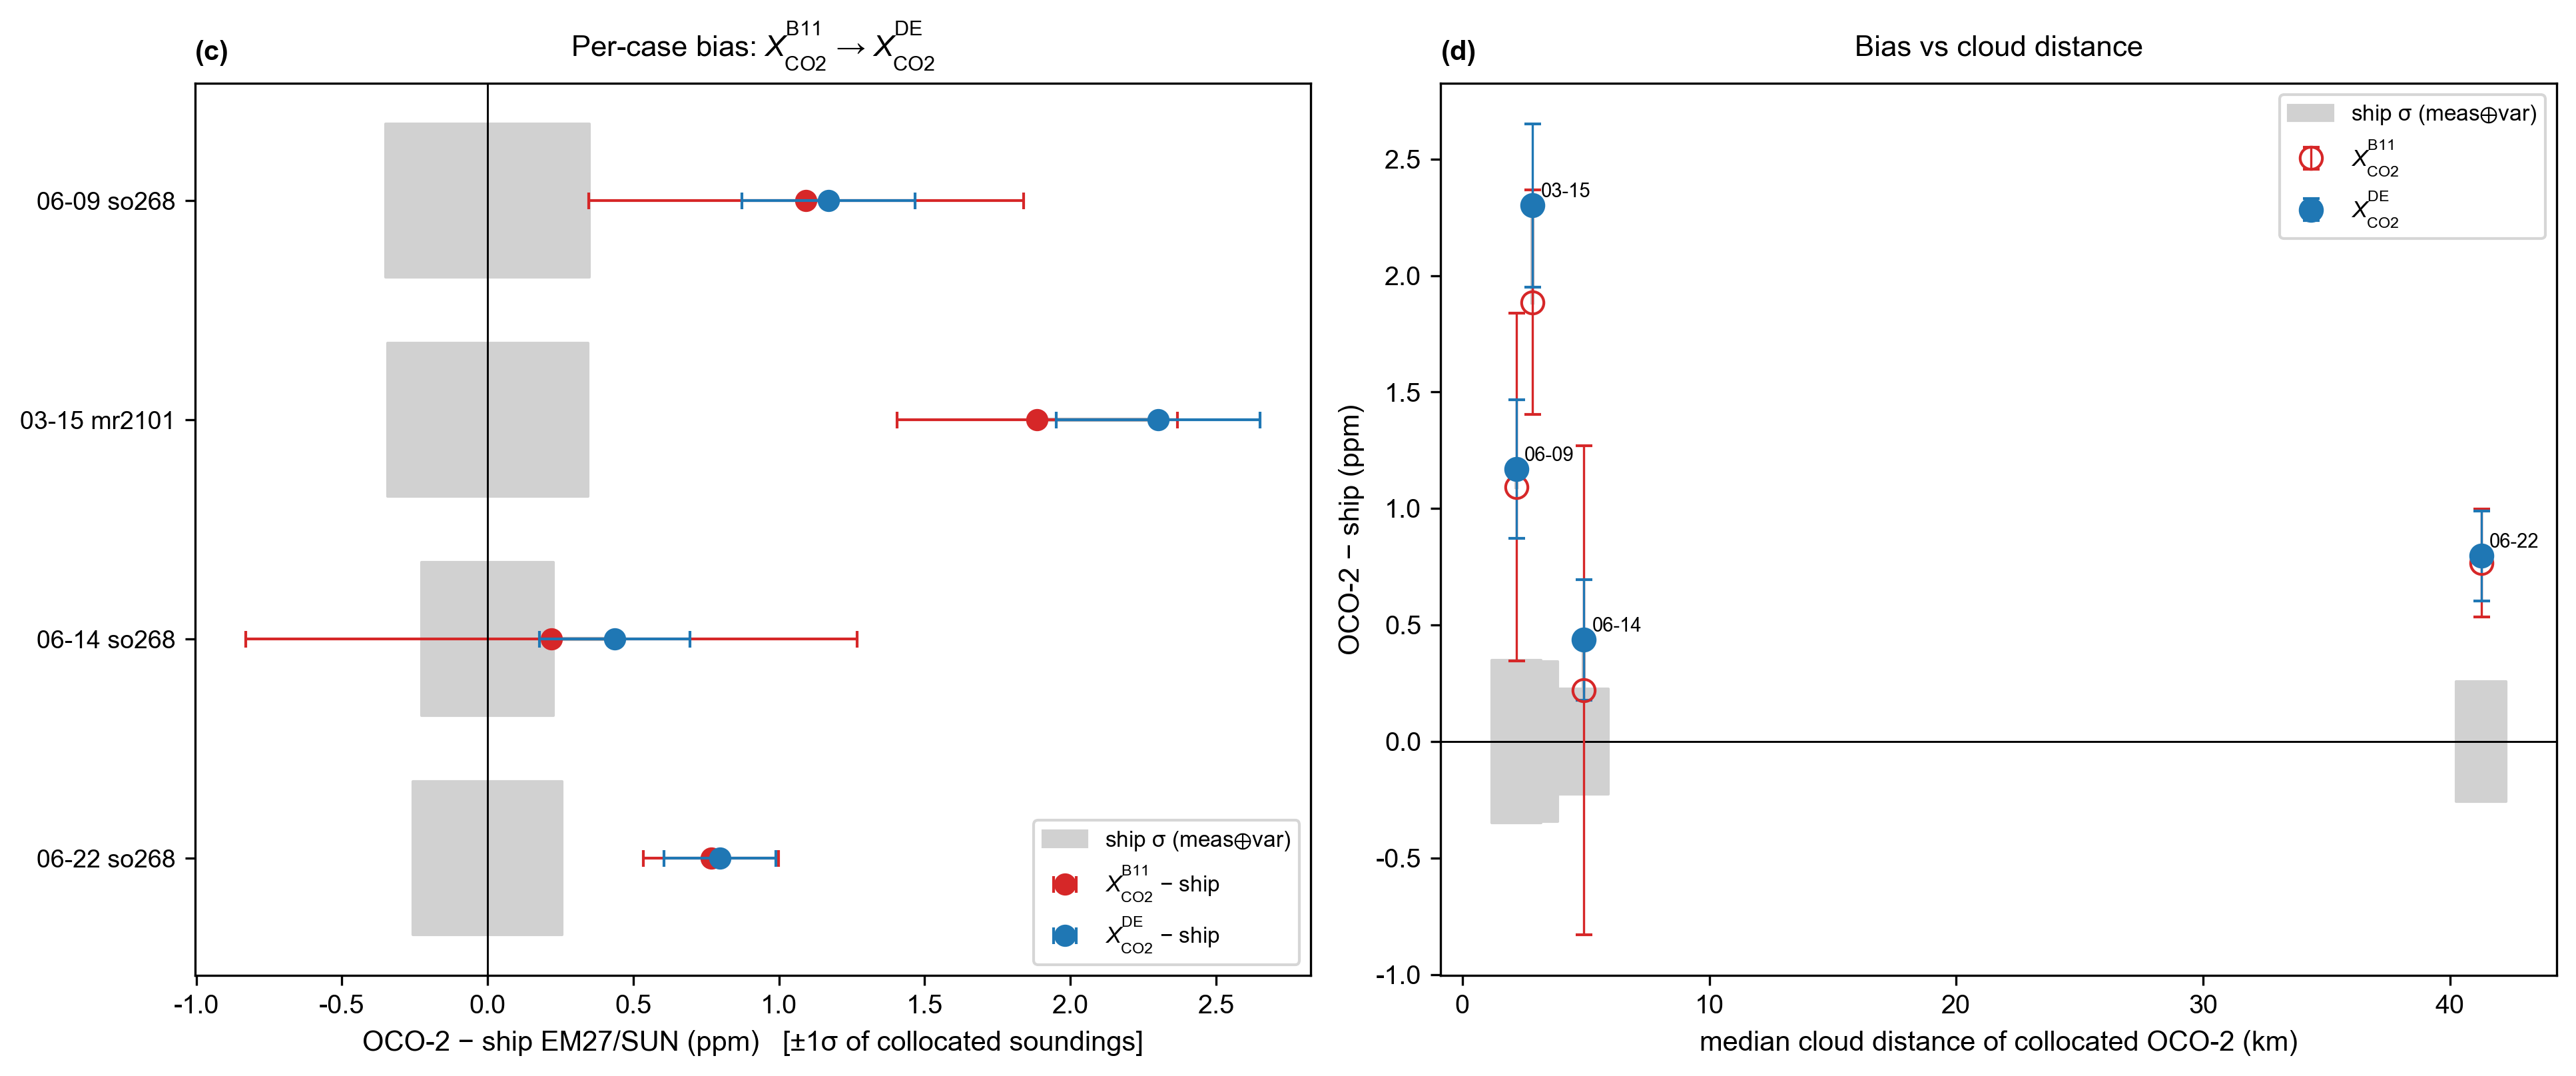
\includegraphics[width=0.95\textwidth]{figures/fig11b_ship_summary.png}
\caption{Independent ocean corroboration. (a, b) ATom aircraft pseudo-column comparison (8 dates, 17 collocated legs, AK-smoothed; the unmeasured stratosphere is filled with the OCO-2 prior so it cancels in the comparison), including the far-cloud negative-control date (9 October 2017): per-leg signed bias before and after correction, and the same residuals against median cloud distance; grey bands mark each leg's own pseudo-column ±1σ. (c, d) Shipborne EM27/SUN comparison (R/V Sonne MORE-2 and R/V Mirai MR21-01; 100 km / ±2 h), including the clear-sky control day (22 June 2019), in the same two views; grey bands mark the ship reference uncertainty (measurement ⊕ within-window variability).}
\label{fig:ocean-validation}
\end{figure}





\FloatBarrier

\subsection{Plume preservation and correction safety}
\label{sec:result-plume}


Local smoothing is primarily attributable to the retrieval-state channel, not to the photon path-length features.


The ~+0.6 ppm enhancement at closest approach to the Westar plant survives the correction essentially unchanged (Fig.~\ref{fig:plume-preservation}a). In the two flagged removal windows, the \ce{O2}A band shifts as strongly as the \ce{CO2} bands (Fig.~\ref{fig:plume-preservation}b) — the all-band fingerprint of cloud contamination rather than of a real plume, whose signature would be confined to the CO2 bands; the worst-case plume signal removable through the spectral channel is ≤ 0.21 ppm.




\begin{figure}[t]
\centering
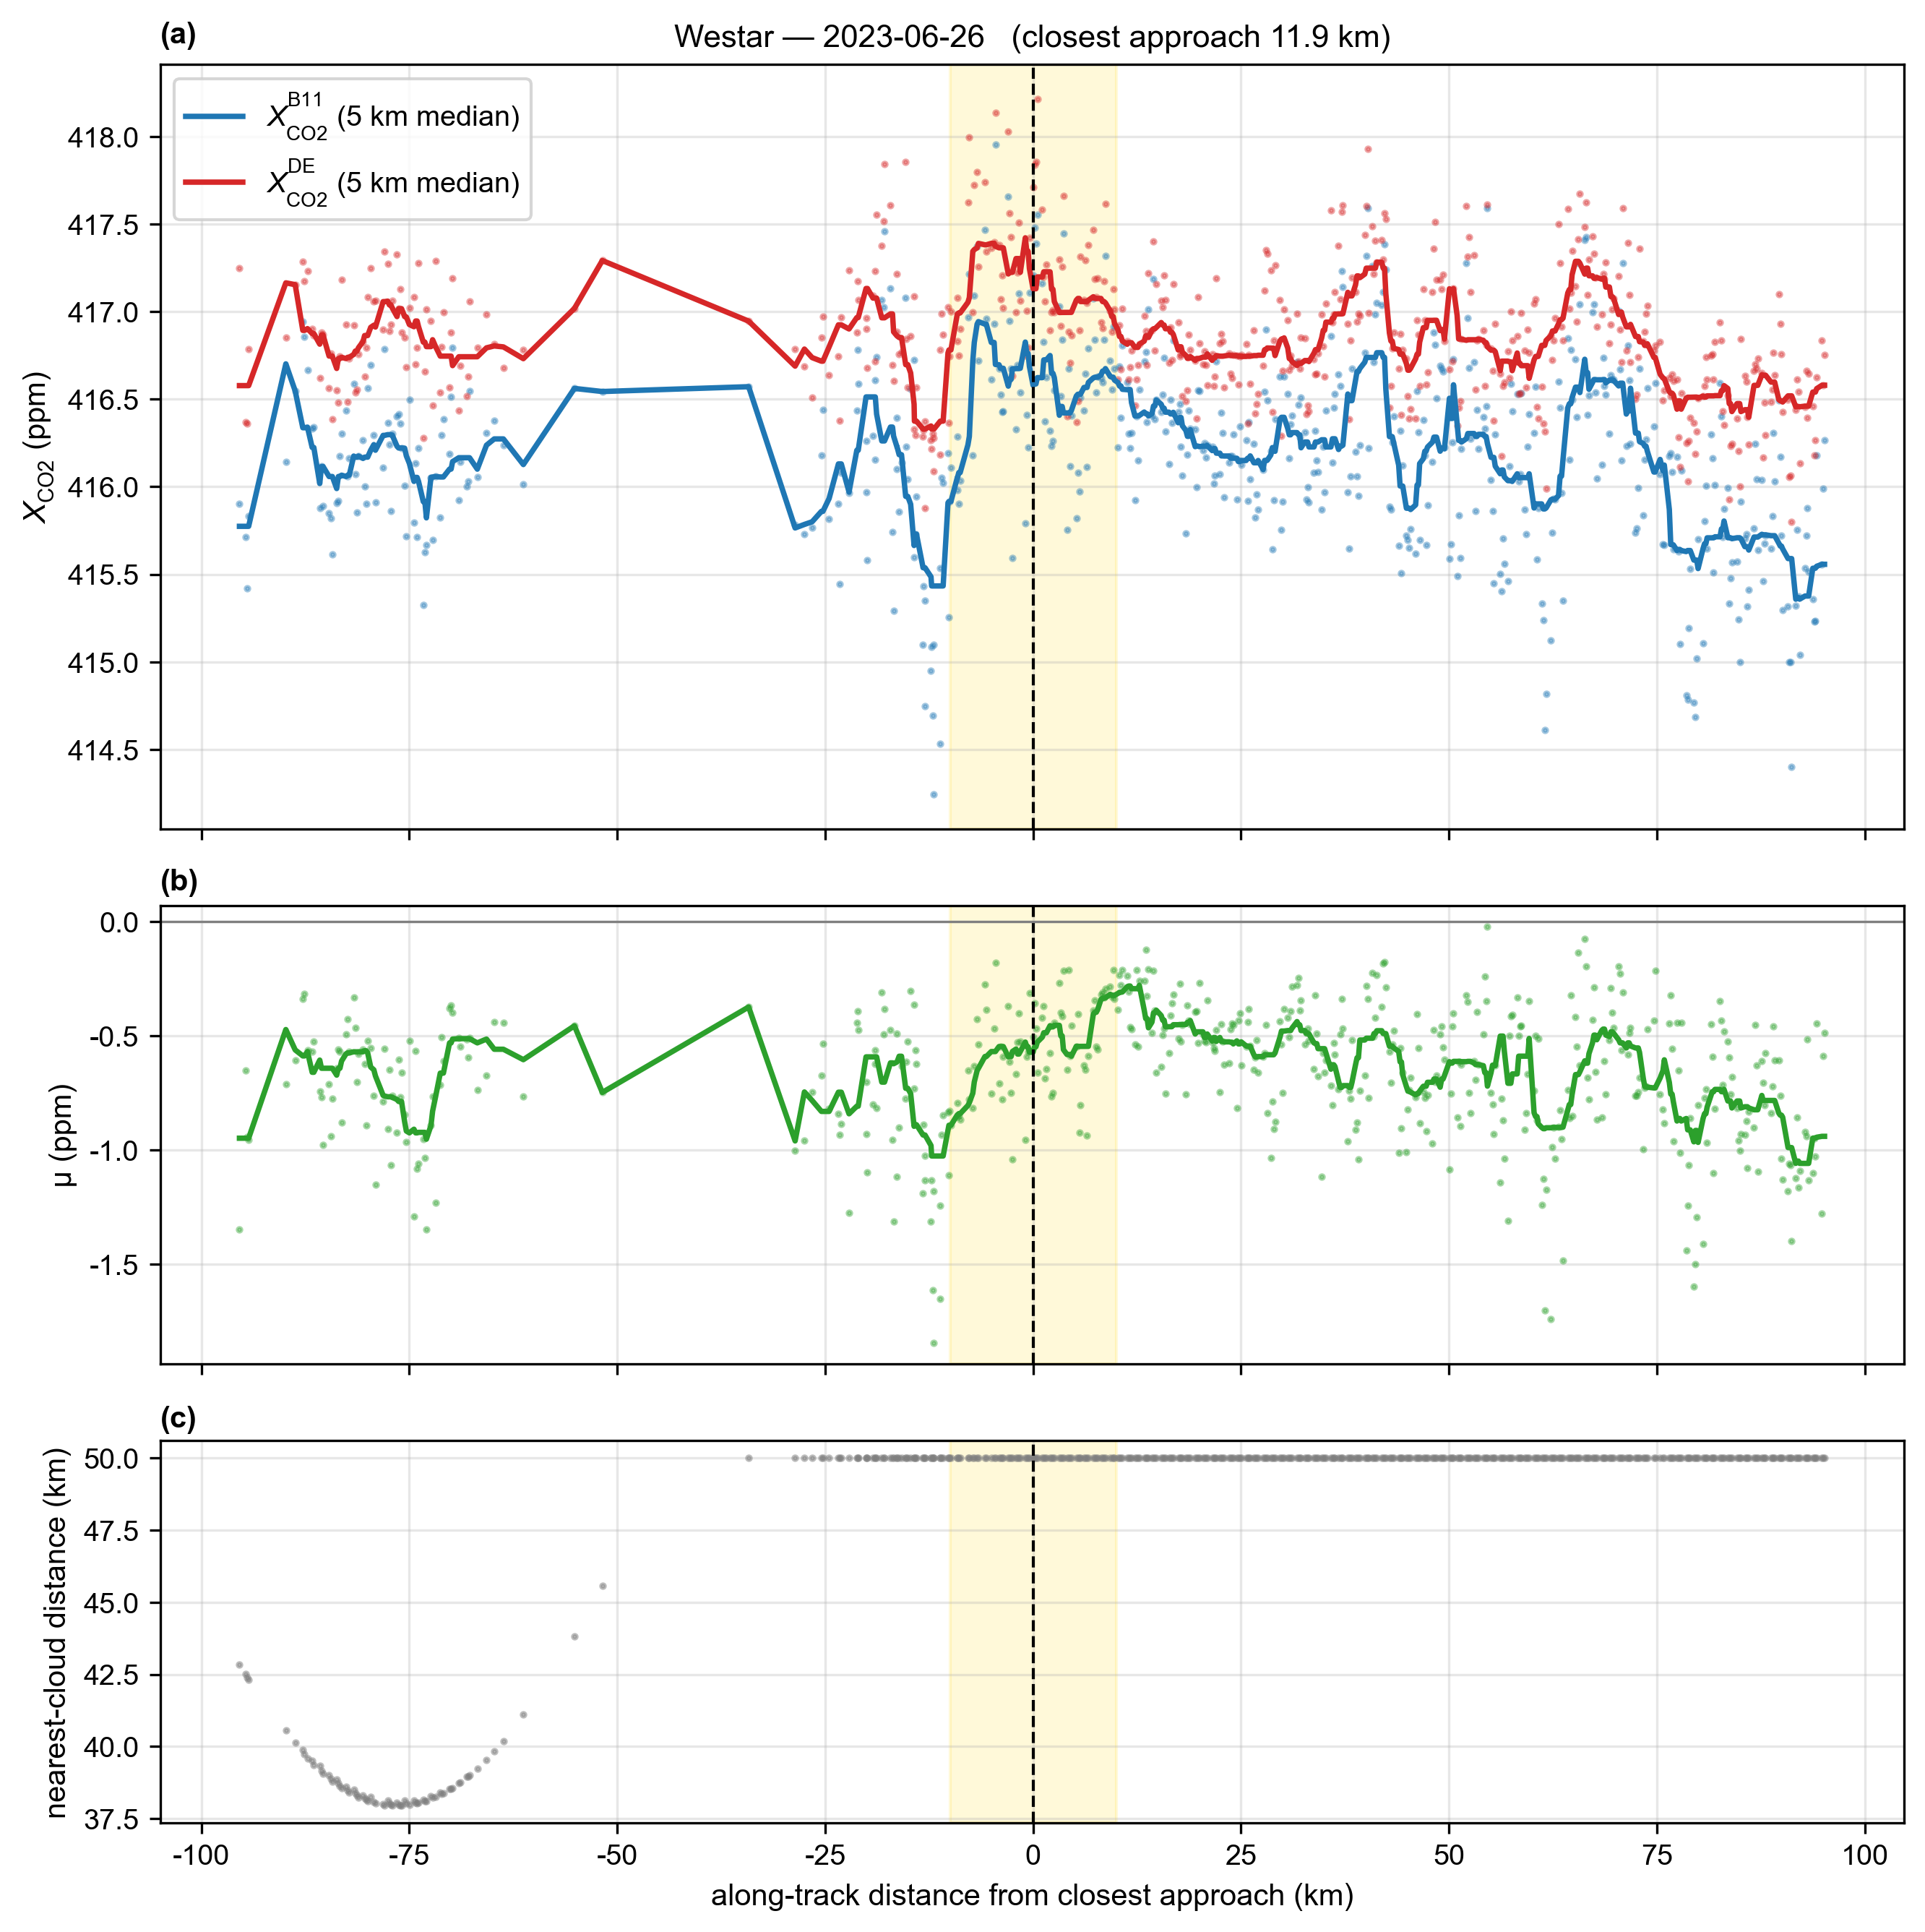
\includegraphics[width=0.65\textwidth]{figures/fig12a_westar_transect.png}\\[4pt]
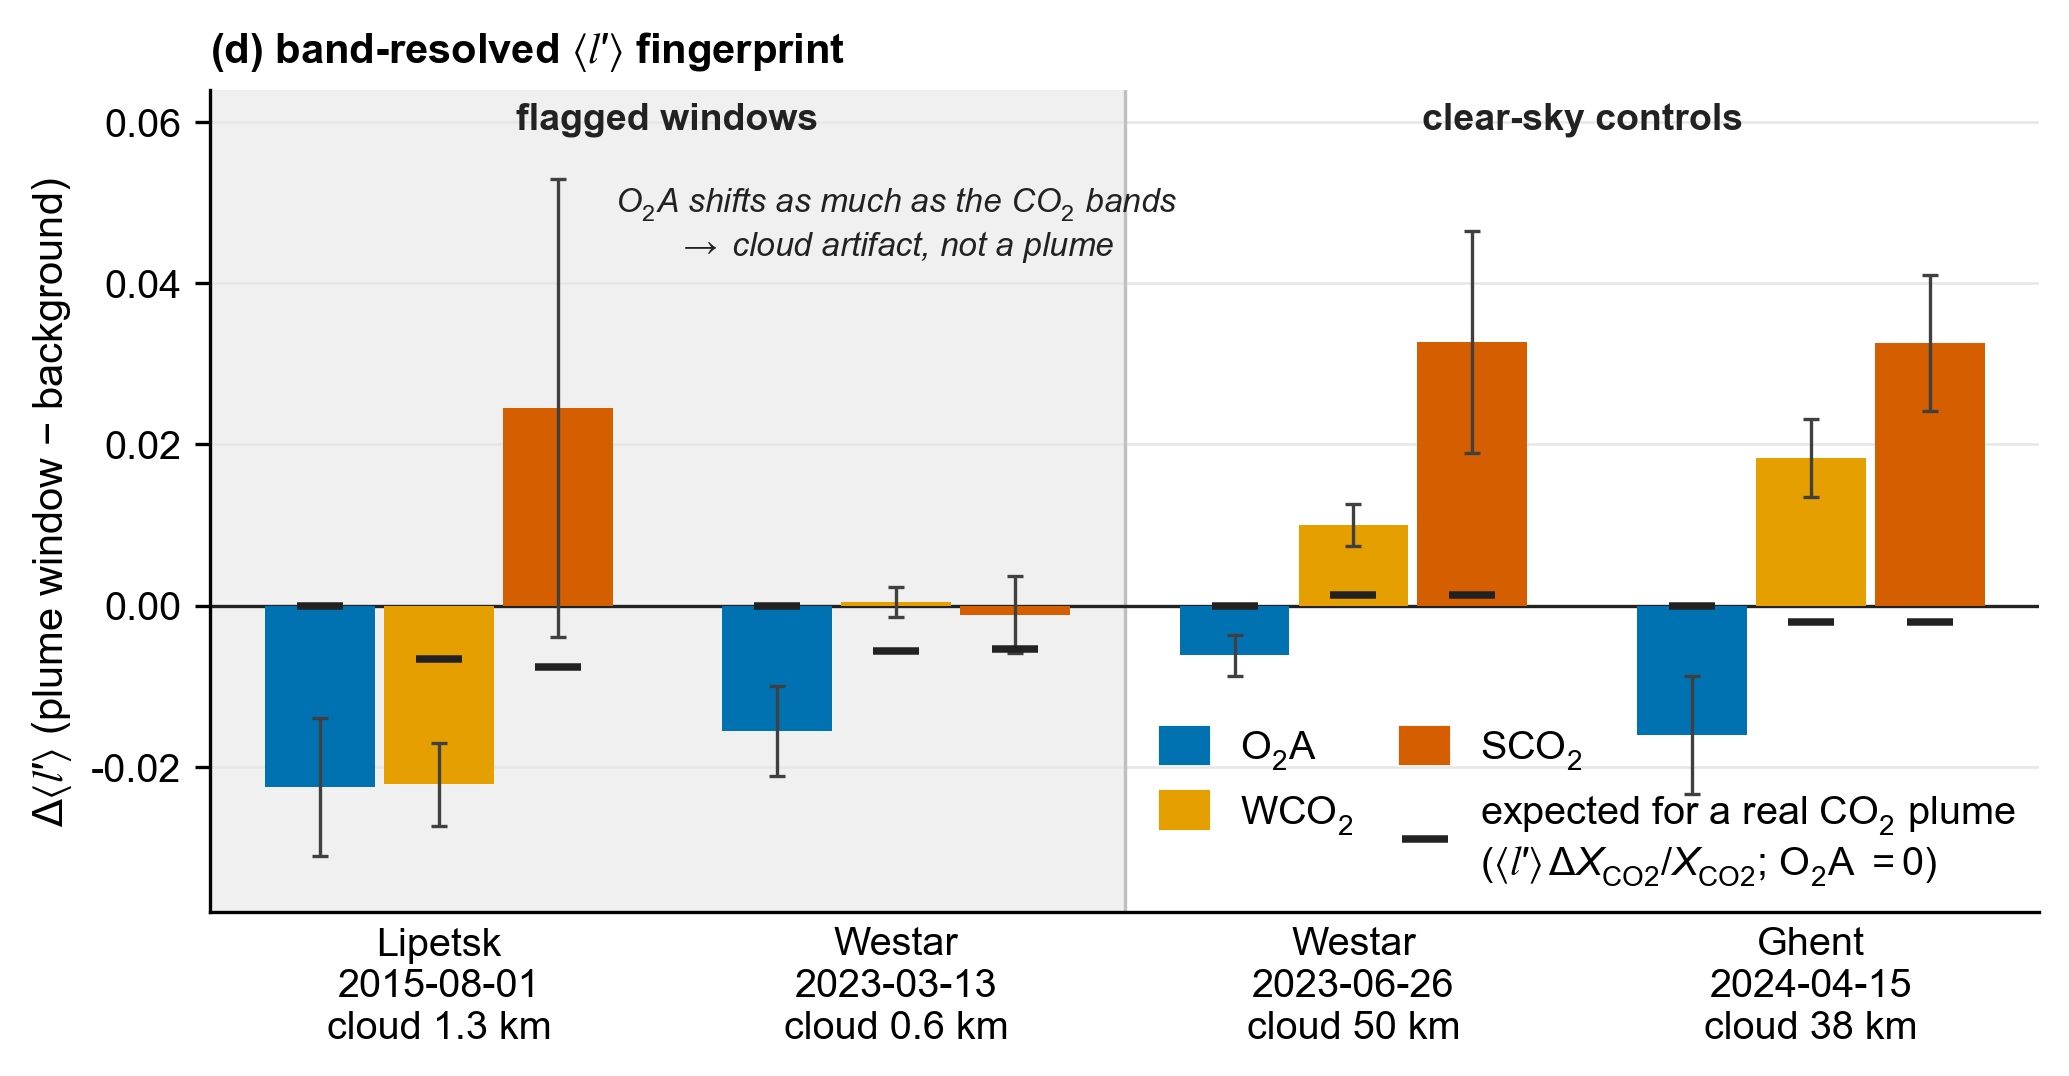
\includegraphics[width=0.65\textwidth]{figures/fig12b_k1_contrast.png}
\caption{Plume preservation and the spectral cloud fingerprint. (a) Along-track transect over the Westar power plant (26 June 2023, clear sky, nearest cloud ≈ 50 km; overpass from the Nassar et al. catalog) before and after correction; lower panels: predicted correction μ and nearest-cloud distance. (b) Band-resolved $\Delta$⟨$l'$⟩ (plume window minus background; ±1 SE) for the two flagged removal windows and two clear-sky controls. Black ticks: signature expected of a real CO2 plume ($\Delta$⟨$l'$⟩ ≈ ⟨$l'$⟩·$\Delta$\xco/\xco in the \ce{CO2} bands via the prior-based optical depth; exactly zero in \ce{O2}A).}
\label{fig:plume-preservation}
\end{figure}




\FloatBarrier

\subsection{Uncertainty and failure modes}
\label{sec:result-unc}




% 4.2 Spectral evidence for a common 3-D mechanism

% Build a three-part evidence chain:

% 1. band- and surface-resolved \(k_1/k_2\) responses with cloud distance;
% 2. the WCO2 land-cover sign rule: savanna approximately \(+0.43\sigma\) and
%    barren approximately \(-0.40\sigma\);
% 3. shadow and brightening branches with opposite XCO2 responses.

% Interpret ocean as the dark endpoint of the cloud–surface contrast axis, but
% label this as a synthesis supported by the observations rather than a closed
% quantitative derivation.

% Use the verified wording:

% > The sign of the WCO2 response follows the measured contrast where land
% > classes straddle the cloud albedo; response magnitudes do not monotonically
% > follow contrast.

% Do not use the superseded “forest sign flip” or “albedo-contrast ordering”
% claims. Close with one RGB case study; move category atlases to the Supplement.

% 4.3 Cross-validated correction performance

% Report random-split inflation versus date-blocked performance, land/ocean and
% near/far-cloud skill, label-noise ceilings, and uncertainty calibration.

% Interpret performance against the estimated ceiling rather than against
% \(R^2=1\): ocean global skill is approximately noise-limited, while land has
% remaining headroom concentrated in the near-cloud regime.

% 4.4 Model comparison and feature attribution

% Present the common-protocol baseline table, emphasizing the difficult
% near-cloud land tail. Then report:

% - the full ensemble performs best overall;
% - `no_spec` is approximately TCCON-neutral;
% - `no_xco2` degrades strongly, particularly for near-cloud land QF1;
% - spectral features remain conditionally informative when the XCO2-departure
%   block is removed.

% State the skill-versus-trust synthesis here for the first time.

% 4.5 Independent TCCON validation

% Use AK-harmonized TCCON as the primary reference and direct TCCON as a
% documented secondary comparison. Report the current production values only
% after regenerating the manuscript table from the frozen tag.

% The paragraph order should be:

% 1. sample and coincidence definition;
% 2. mean absolute bias and footprint RMSE;
% 3. number of improved station-days;
% 4. Wilcoxon and site-clustered bootstrap results;
% 5. radius/window and QF0/QF1 sensitivity;
% 6. high-latitude and worsening cases.

% Keep direct-reference results nearby but do not let the dual-reference
% explanation obscure the AK-harmonized primary result.

% 4.6 Distinguishing correction from smoothing

% Place the feature-free smoother immediately after TCCON:

% - it reduces footprint scatter more than the model;
% - it leaves station-day bias nearly unchanged;
% - the model reduces both bias and RMSE.

% This establishes that the validation improvement is not merely local
% denoising.

% 4.7 Ocean validation and far-cloud controls

% Present ATom, shipborne EM27/SUN, and the far-cloud/clear-day cases where the
% correction is nearly inert. Treat these as independent corroboration, not as
% equivalent in statistical weight to TCCON. State the limited sample and
% reference-scale caveats.

% 4.8 Plume preservation and correction safety

% Report:

% - matched control-window nulls;
% - the preserved Westar transect enhancement;
% - the all-band versus CO2-band \(k_1\) discriminator;
% - the spectral-channel removal bound of at most 0.21 ppm in the worst tested
%   case and at most 0.01 ppm in clear cases;
% - approximately 55% [40–63%] removal of plume-free local spread by the full
%   model, 54% by `no_spec`, and 29% by `no_xco2`.

% The required interpretation is:

% > Local smoothing is primarily attributable to the retrieval-state channel,
% > not to the photon path-length features.

% 4.9 Uncertainty and failure modes

% End Results by defining the boundary of reliability:

% - random-effects residual offset and its reference-scale interpretation;
% - representation error increasing with coincidence radius;
% - under-dispersed whole-budget uncertainty if between-case variance is
%   omitted;
% - bright surfaces as the main footprint-level failure stratum;
% - high-latitude residuals as station-day bias failures;
% - predictive uncertainty as a useful land-failure indicator that cannot
%   remove reference-scale bias.